\chapter{下丘脑:生存的自动控制、激素控制和行为控制} \label{chap:chap41}

个体的生存需要严格控制体温、水平衡和血压,以及充足的食物摄入和适当调节睡眠/觉醒周期。
一个物种的生存需要个体的生育、交配和养育后代,同时,在适当的情况下,对他人的攻击行为也是一种适应性表现。
下丘脑中的神经元控制所有这些关键的生存活动。


正如我们将在本章中了解到的那样,下丘脑和大脑中相互关联的区域通过募集适当的行为和生理反应来应对身体和情绪上的挑战。
这些活动的协调确保了内部环境的稳定性,这一过程称为\textit{内稳态}。
下丘脑作用于三个主要系统:自动运动系统、神经内分泌系统和介导动机行为的神经通路。


自动运动系统不同于控制骨骼肌的躯体运动系统。
躯体运动神经元调节横纹肌的收缩(第~\ref{chap:chap31}~章),而自主运动神经元则通过与平滑肌细胞和心肌细胞、具有内分泌和外分泌功能的腺体细胞以及脂肪细胞等代谢目标的突触来调节血管、心脏、皮肤和内脏器官。
神经内分泌系统的工作方式不同,它从位于下丘脑正下方的垂体(“主腺”)分泌几种肽类激素。
这些垂体激素控制肾脏的保水、分娩、哺乳、体细胞生长、配子发育,以及从三个下游腺体(性腺、肾上腺皮层和甲状腺)释放非肽激素。


尽管自动神经响应和神经内分泌响应在很大程度上是非意识的,但它们与躯体运动系统执行的自动行为紧密结合。
跑步、攀登和举重等自主行为均会产生代谢、心血管和体温调节等结果。
这些需求由\textit{自动神经系统}和神经内分泌系统通过心肺驱动、心输出量、局部血流、散热和燃料动员的变化自动满足这些需求。
这种补偿性变化主要是通过前馈中枢指令实现的,辅之以感官反馈激活的反射。
同样,情绪状态会引起自动神经和神经内分泌反应。
恐惧、愤怒、快乐和悲伤的感觉具有特有的自动神经和荷尔蒙表现。


在本章中,我们首先探讨\textit{内稳态}的概念及其实现的一般方法。
然后我们讨论下丘脑及其两个“非自主”运动臂的解剖学和功能组织:\textit{自动神经系统}和神经内分泌系统。
之后,我们将深入研究下丘脑稳态控制的三个经典例子:调节体温、水平衡及其相关缺乏的驱动力、口渴,能量平衡及其驱动力、饥饿。
我们通过检查下丘脑的性二态区域及其在调节性行为、攻击性和育儿方面的作用来得出结论。
有关睡眠周期和昼夜节律调节的更多讨论,请参见第~\ref{chap:chap44}~章。



\section{\textit{内稳态}将生理参数保持在一个狭窄的范围内,这对生存至关重要}

19 世纪中叶,身体内部环境在广泛的行为状态和外部条件下的稳定性吸引了法国生理学家和实验医学创始人\textit{克劳德$\cdot$伯纳德}的注意力。
他写道:“\textit{内环境}是独立生存的必要条件。” 
基于这个想法,在 1930 年代,美国生理学家\textit{沃尔特$\cdot$坎农}引入了\textit{内稳态}的概念来描述维持体液成分、体温、血压和其他生理变量的恒定性机制,所有这些是生存所必需的。


稳态机制具有高度适应性,因为它们极大地扩展了可以耐受的条件范围。
例如,在运动过程中,许多参数会显著增加:心输出量增加 4 到 5 倍,氧气和燃料消耗增加 5 到 10 倍,产热量增加到类似的程度。
在没有\textit{补偿反应}的情况下,血压会随着心脏输出量的增加而增加,从而导致血管破裂;
循环燃料将降至极低水平,使能量细胞挨饿;
高温会使细胞蛋白质变性。
事实上,\textit{内稳态}的能力是非凡的,这使得动物能够在季节性温度可能波动 70°C 的高纬度地区生存,并使人类能够在极热的撒哈拉沙漠的沙滩上奔跑 251 公里(撒哈拉沙漠马拉松赛)。
稳态机制极大地扩展了可以生存的栖息地、活动和创伤的范围。


\textit{内稳态}需要来自身体的负面感觉反馈。
反馈回路的概念源于传感器的发现,这些传感器检测关键的生理变量,然后将它们与行为、自动神经和神经内分泌运动输出相结合。
借鉴负反馈控制的工程原理,这产生了生理“设定点”有助于控制体温、血液渗透压、血压和体脂含量等关键参数的概念。


设定点模型很有吸引力,因为恒温器在将室温保持在目标设定点方面非常有效,并且通过类比,体温等生理变量同样受到严格控制。
如图~\ref{fig:41_1}A~所示,在此类模型中,参数存在一个“设定点”,在体温的情况下为 37°C,并且在任何给定时刻,都会评估参数的实际水平,并通过反馈和误差检测与目标设定点进行比较。
任何高于或低于的偏差都会触发抵消纠正反应:如果太热,皮肤血管扩张、出汗和在游泳池里泡一泡;
如果太冷,血管收缩、产热、发抖和穿毛衣。
对于体温调节,设定点和误差检测历来被视为下丘脑\textit{视前区}神经元的涌现特性。


\begin{figure}[htbp]
	\centering
	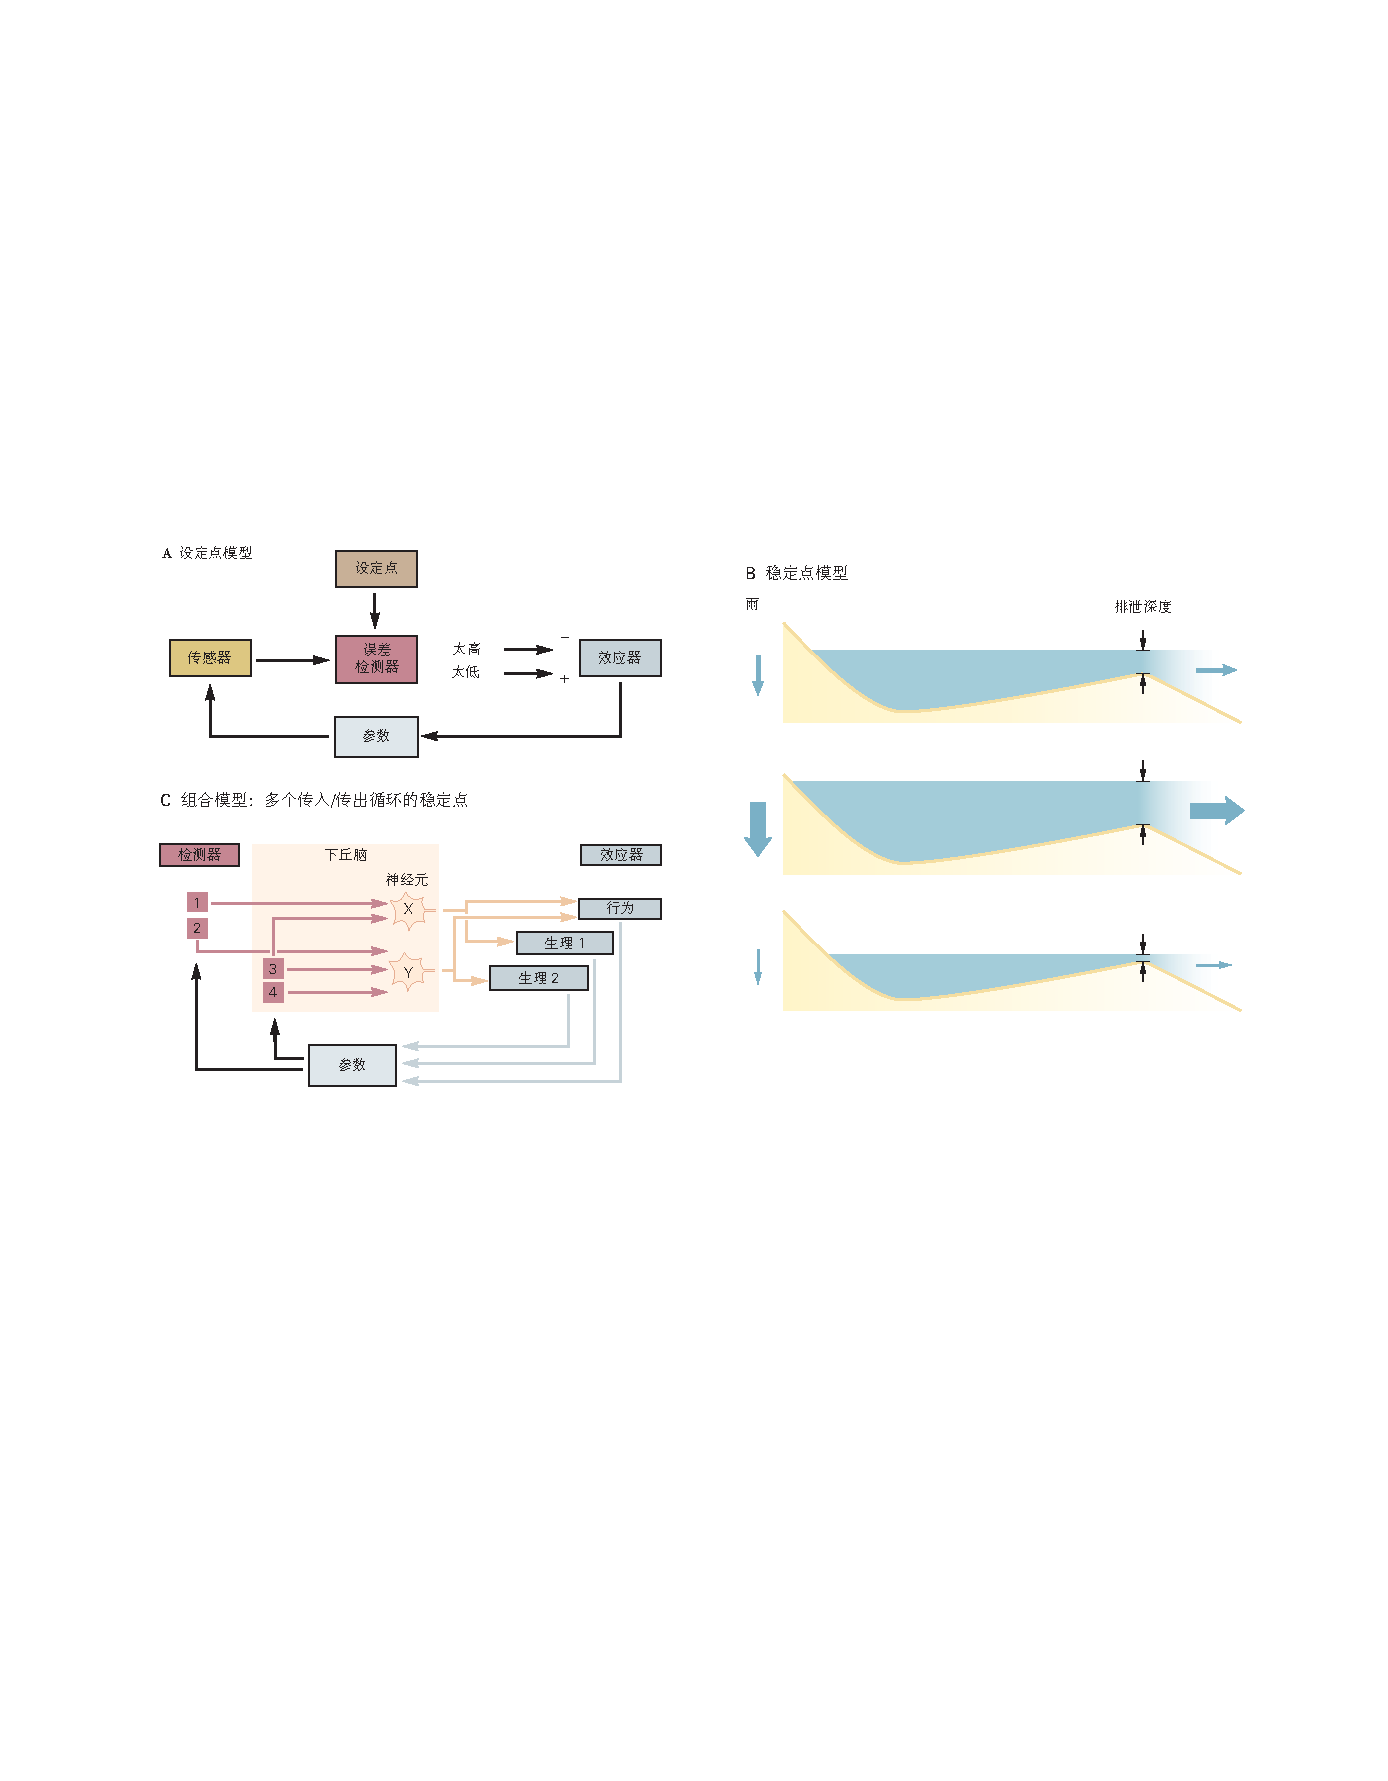
\includegraphics[width=1.0\linewidth]{chap41/fig_41_1}
	\caption{设定点、稳定点和\textit{内稳态}。
		A. \textit{设定点}视图的灵感来自工程原理。
		与恒温器一样,通过提供参数现有水平的反馈,确定它与理想化设定点的比较,然后采取纠正措施将参数恢复到设定点,可以实现恒温。
		虽然流行多年,但由于多年的研究未能发现编码设定点和执行误差检测的分子和神经基础,它已经失宠。
		B. \textit{稳定点模型}的灵感来自于观察到许多系统在没有任何反馈或错误检测的情况下实现稳定。
		在这个例子中,从湖中流出的水位与湖的深度成正比。
		下雨时,湖水位的升高或降低会导致或多或少的水从湖中流出。
		在没有设定点或错误检测的情况下,湖的水位保持相当恒定。
		一个相关的例子是体重的调节。
		食物摄入量增加会导致体重增加。 随着体重的增加,携带和维持增加的体重所消耗的能量也会增加。
		正因为如此,体重也应该有它的稳定点\cite{speakman2011set}。
		C. 在该模型中,A 部分的反馈概念和 B 部分的稳定点概念相结合。
		明显的设定点实际上是稳定点,是多个反馈通知传入/传出环路的涌现特性。}
	\label{fig:41_1}
\end{figure}


随着时间的推移,设定点模型需要修改,因为深入调查未能发现任何用于编码设定点和执行错误检测的分子或神经元基础。
此外,如图~\ref{fig:41_1}B~所示,原则上可以在没有\textit{设定点}、反馈或误差检测的情况下实现“类似设定点”的调节,即所谓的“\textit{稳定点}”模型。
考虑湖泊水位的变化。
当降雨过多时,水位会上升;
排干湖水的河流水位上升,流量增加。
当降雨量少时,情况恰恰相反。
因此,排干湖泊的河流不断变化的流量将其水位保持在稳定点附近,而无需理想化的设定点、反馈或错误检测。
虽然\textit{稳定点模型}的各个方面都很有吸引力,但它也是不完整的,因为稳态过程清楚地接收到有关干扰的重要反馈,并且这种反馈会产生加速恢复的重要反应。
正如我们将要看到的,温度、渗透压和身体脂肪会被直接或间接地“感知”,这会影响下丘脑中产生抵消反应的神经元的活动。


今天大多数生理学家都采用了“分布式稳定点”模型,该模型结合了对多个感觉/效应器回路的强大反馈控制(图~\ref{fig:41_1}C)。
例如,对于体温,没有单一的特定设定点,大脑中也没有对单一设定点进行编码和错误检测的位置;
简而言之,没有恒温器。
相反,有多个温度探测器位于不同的部位(皮肤、核心和大脑),每个探测器都通过神经通路耦合,这些神经通路穿过视前区,到达不同的体温效应器(皮肤血管、汗腺、棕色脂肪) 新陈代谢、颤抖和行为通路)。
当参与时,这些效应器中的每一个都会影响体温。
体温的表观设定点实际上是由多个反馈通知传入/传出环路的组合活动产生的紧急稳定点。
正如我们稍后将看到的,这种微妙的模型也适用于血压、血液渗透压和体脂的调节。


\begin{table}[htbp]
	\caption{下丘脑整合与六种生命功能相关的行为(躯体运动)、自动和神经内分泌反应} \label{tab:41_1} \centering
	\begin{tabular}{l}
		\toprule
		疾病 \\
		\midrule
		\makecell[l]{1. \textit{血压和电解质成分}。下丘脑调节口渴、食欲和饮酒行为;\\血管舒缩张力的自动控制;以及激素如血管加压\\素的释放(通过室旁核)。}  \\
		\makecell[l]{2. \textit{能量代谢}。下丘脑调节饥饿和进食行为、\\消化的自动控制以及糖皮质激素、生长激素和促甲状腺激素等激\\素的释放(通过弓形核和室旁核)。}  \\
		\makecell[l]{3. \textit{生殖(性和父母)行为}。下丘脑控制生殖器官的自动调节和性腺的\\内分泌调节(通过视前内侧核、腹内侧\\核和腹侧核)。}  \\
		\makecell[l]{4. \textit{体温}。下丘脑影响体温调节行为(寻求更温暖或更凉爽的环境),\\控制自动体温保持/丧失机制,并控制影\\响代谢率的激素分泌(通过视前区)。}  \\
		\makecell[l]{5. \textit{防御行为}。下丘脑调节对环境中的威胁(如捕食者)的应激反应\\和战斗或逃跑反应(通过室旁核、下丘脑\\前核和背侧前核以及下丘脑外侧区)。}  \\
		\makecell[l]{6. \textit{睡眠-觉醒周期}。下丘脑调节睡眠-觉醒周期\\(通过视交叉上核的昼夜节律时钟)和觉醒时的唤醒水平(通过\\下丘脑外侧区和结节乳头核)。}  \\
		\bottomrule
	\end{tabular}
\end{table}

\section{下丘脑协调稳态调节}

下丘脑将生理参数的状态与行为、自动神经和神经内分泌运动系统的输出相结合,从而调节六种重要的生理功能(表~\ref{tab:41_1})。
如图~\ref{fig:41_2}~所示,下丘脑位于大脑底部,紧靠垂体上方。
它的前部(嘴侧)以布洛卡斜带为界;
背侧由前连合、终纹床核、不确定带和丘脑组成;
和后部(尾部)由腹侧被盖区和脚间核组成。


\begin{figure}[htbp]
	\centering
	\includegraphics[width=0.94\linewidth]{chap41/fig_41_2}
	\caption{下丘脑的结构。
		A. 下丘脑的正面视图(沿平面 A 的截面显示在右上角的大脑矢状视图中)。
		第三脑室在中线;
		与心室相邻的室旁核、背内侧核和弓状核在此水平形成神经内分泌运动区和脑室周围区。
		腹内侧核是下丘脑核内侧柱的一部分,下丘脑外侧区域是此处显示的下丘脑部分的外侧区域成分。 
		B. 下丘脑核内侧柱的矢状面(头尾之间的)视图,显示相邻的(尾部)黑质和中脑的腹侧被盖区。
		表~\ref{tab:41_1}总结了关键下丘脑核团的功能意义。}
	\label{fig:41_2}
\end{figure}



\subsection{下丘脑通常分为头尾之间的三个区域}

下丘脑区域根据它们在尼氏染色切片中的位置和外观来命名。
下丘脑从头端到尾端分为三个区域。
(1)视前下丘脑位于视交叉上方,包含控制水平衡和口渴、温度、睡眠、性行为和昼夜节律的神经元。
(2)下丘脑结节位于垂体上方,包含控制垂体激素分泌、自动神经流出和各种行为(包括饥饿、性行为和攻击行为)的神经元。
(3)后下丘脑包括后核和乳头核,以及影响觉醒的结节乳头核中的组胺能神经元。
下丘脑后部区域其他神经元的功能不太明确。


\textit{下丘脑外侧区}从中部跨越到下丘脑尾部。
与维持\textit{内稳态}和特定生存行为相比,它与奖励通路和唤醒的联系更紧密。
事实上,它与伏隔核和腹侧被盖区密切相关,这两个区域涉及奖励(第~\ref{chap:chap43}~章),并且包含广泛投射到整个皮层的神经元。
最后,表达神经肽食欲素(\textit{下视丘分泌素})的\textit{下丘脑外侧区}神经元在稳定觉醒方面发挥着关键作用(第~\ref{chap:chap44}~章)。



\subsection{模态特异性下丘脑神经元将内感受性感觉反馈与控制适应性行为和生理反应的输出联系起来}

几十年来已经出现了下丘脑功能的一般原则。
当稳态控制下的参数受到干扰时,外围和大脑中的神经元会做出反应。
这样的神经元可以直接响应刺激或间接响应激素和其他跟踪调节参数的因素的变化。
然后将这种感觉信息传递到下丘脑内特定部位(或多个部位)中功能适当的调节神经元。
一旦信息被下丘脑神经元整合,结果就会向下游传递到控制特定行为和生理反应的运动回路。
结果是协调的纠正反应(例如,寻求温暖加上热量的产生和保留,口渴加上肾脏的水分保留,或饥饿加上减少的能量消耗)。


我们对下丘脑神经元功能的理解最近在活跃的动物中使用光遗传学和化学遗传学技术得到了改进。
通过选择性地激活下丘脑神经元的子集,即使在完全没有需要的情况下,也可以唤起特定的行为和生理反应。
体温的关键调节神经元位于\textit{视前正中核}。
如图~\ref{fig:41_2}A~所示,水平衡由三个部位的神经元调节(\textit{视前正中核}、\textit{终板血管器官}和\textit{穹窿下器})以及弓状核中神经元的能量平衡。



\subsection{模态特异性下丘脑神经元也接收关于预期稳态挑战的下行前馈输入}

除了来自提供关于身体状态的重要反馈的感觉信号的输入外,下丘脑中的关键调节神经元还接收来自神经元的“自上而下”的前馈输入,这些神经元预测未来的稳态挑战。
例如,当食物匮乏的动物检测到预测食物供应的线索时,甚至在食物被摄入之前,弓状核中促进饥饿的神经元的放电就会迅速下降。
这种自上而下的前馈控制让身体为预期的稳态挑战做好准备。
此外,这种快速调节,通过对抗以缺乏驱动神经元的高活性为代表的厌恶状态,对于激发基于缺乏的行为(如口渴和饥饿)可能很重要(下面讨论)。


接下来,我们检查下丘脑的两个效应臂:自动运动系统和神经内分泌系统。



\section{自动系统将大脑与生理反应联系起来}

尽管自动运动系统执行许多由下丘脑发起的生理反应,但自动系统也受脑干和脊髓回路的调节(第~\ref{chap:chap40}~章)。
因此,自动神经功能对下丘脑的依赖程度也有所不同。
例如,排尿在很大程度上独立于下丘脑,而血压调节在很大程度上取决于脑干中的回路,但也可以由下丘脑调节。
相比之下,\textit{棕色脂肪组织}的产热作用很大程度上受制于下丘脑。



\subsection{自动系统中的内脏运动神经元被组织成神经节}

与运动神经元位于腹侧脊髓和脑干的躯体运动系统不同,自动运动神经元的细胞体存在于称为神经节的周围神经扩张中。
自动运动神经元支配腺体、平滑肌、心肌和脂肪组织中的分泌上皮细胞。


1880 年,英国的\textit{沃尔特$\cdot$盖斯凯尔}开始努力理解自动神经节的组织原理,后来由\textit{约翰$\cdot$兰里}继续努力。
他们刺激自动神经并观察终末器官的反应(例如,血管收缩、\textit{寒毛直立}、出汗、瞳孔收缩)。
他们使用尼古丁来阻断来自单个神经节的信号,以测试神经节之间的相互作用。
\textit{兰里}提出,特定的化学物质必须由自动神经节的节前神经元释放,并且这些物质通过与靶向终末器官的节后神经元上的受体结合而起作用。
这些想法为后来的化学突触传递研究奠定了基础。
\textit{兰里}还区分了\textit{自动神经系统}和躯体运动系统,并以此创造了我们目前的大部分命名法。


\begin{figure}[htbp]
	\centering
	\includegraphics[width=0.75\linewidth]{chap41/fig_41_3}
	\caption{外周自动神经通路中的不同类型细胞选择性地控制具有不同表型的靶细胞。
		自动运动神经元位于中枢神经系统之外的神经节中,由脊髓和脑干中的神经节前神经元控制。
		副交感神经节和交感神经节内的这些下游神经元调节三种类型的效应细胞:平滑肌、腺体细胞和心肌。
		此外,仅在交感神经节中发现的下游神经元选择性地控制淋巴组织中的棕色脂肪细胞和免疫细胞。
		该图说明了控制功能的三种基本细胞类型:节前神经元、下游神经节神经元和不同的靶效应细胞。}
	\label{fig:41_3}
\end{figure}


\textit{自动神经系统}分为三个部分:
交感神经、副交感神经和肠神经。
交感神经节和副交感神经节中的所有神经元都由节前神经元控制,节前神经元的胞体位于脊髓和脑干。
如图~\ref{fig:41_3}~所示,节前神经元合成并释放神经递质\textit{乙酰胆碱},后者作用于节后神经元上的烟碱\textit{乙酰胆碱}受体,产生快速兴奋性突触后电位和起始动作电位,这些电位传播到末端器官中与效应细胞的突触。
交感神经系统和副交感神经系统通过五个标准进行区分:

1. 它们在脊髓和脑干中节前神经元的节段组织。

2. 它们神经节的外围位置。

3. 它们所支配的终末器官的类型和位置。

4. 它们对终末器官产生的作用。

5. 其节后神经元所使用的神经递质。



\subsection{节前神经元位于脑干和脊髓的三个区域}

如图~\ref{fig:41_4}~所示,副交感神经通路起源于脑干中的颅神经区和脊髓骶段中的第二区。
这些副交感神经区围绕着在脊髓的胸段和腰段连续延伸的交感神经区。


\begin{figure}[htbp]
	\centering
	\includegraphics[width=1.0\linewidth]{chap41/fig_41_4}
	\caption{自动运动系统的交感神经和副交感神经分区。
		交感神经节靠近脊柱,几乎供应身体的每个组织。
		一些组织,例如骨骼肌,仅通过其动脉血供间接受到调节。
		副交感神经节位于其目标附近,不包括皮肤或骨骼肌。}
	\label{fig:41_4}
\end{figure}


颅副交感神经通路起源于四个颅神经的一般内脏运动核中的节前神经元:
中脑和面部(N. VII)中的动眼神经(N. III),舌咽神经(N. IX)和迷走神经(N. X) 在髓质中。
颅副交感神经核与混合颅神经(例如面神经、舌咽神经和迷走神经)一起在第~\ref{chap:chap40}~章中进行了描述。
脊髓副交感神经通路起源于骶段 S2-S4 的节前神经元。
它们的细胞体位于灰质的中间区域,它们的轴突通过腹根投射到周围神经中。


如图~\ref{fig:41_4}~所示,交感神经节前细胞柱在脊髓的颈椎和腰骶部之间延伸,对应于第一胸段和第三腰段。
交感神经节前神经元的胞体大部分位于中间外侧细胞柱;
其他位于中央管周围的中枢自动区和连接中枢区与中间外侧细胞柱的带中。
如图~\ref{fig:41_5}~所示,节前交感神经元的轴突从脊髓通过最近的腹侧根伸出,然后与称为交感支的小连接神经一起运行,然后终止于椎旁交感神经链中的节后细胞。


\begin{figure}[htbp]
	\centering
	\includegraphics[width=1.0\linewidth]{chap41/fig_41_5}
	\caption{交感神经流出被组织成椎旁和椎前神经节组。
		脊髓节前细胞的轴突通过腹根和椎旁交感神经链到达节后神经元。
		轴突要么在椎旁神经节的节后神经元上形成突触,要么从链条中投射到内脏神经中。
		内脏神经中的节前轴突与椎前神经节中的节后神经元和肾上腺髓质中的\textit{嗜铬细胞}形成突触。}
	\label{fig:41_5}
\end{figure}


\subsection{交感神经节投射到全身的许多目标}

如图~\ref{fig:41_4}~所示,交感神经运动系统通过影响全身几乎每个组织内的靶细胞来调节全身生理参数,例如血压和体温。
这种调节取决于来自脊髓和控制节前神经元活动的脊髓上结构的突触输入。


激发节前交感神经活动的重要脊髓上神经元群位于延髓头端腹外侧、脑干中的苍白中缝和下丘脑中的室旁核。
如图~\ref{fig:41_5}~所示,节前神经元将这些下行输入与局部节段性感觉输入整合在一起,并与椎旁和椎前交感神经节中的神经元形成突触。


神经节神经元反过来与各种终末器官形成突触,包括血管、心脏、支气管气道、立毛肌、棕色脂肪以及唾液腺和汗腺。
交感神经元还通过投射到骨髓和胸腺中的初级淋巴组织以及脾脏中的次级淋巴细胞来调节免疫功能。
如图~\ref{fig:41_5}~所示,肾上腺髓质中\textit{嗜铬细胞}上节前神经元突触的一个子集,它们将\textit{肾上腺素}和\textit{去甲肾上腺素}分泌到循环中作为激素作用于远处的目标。


椎旁和椎前交感神经节在位置和组织上都不同。
椎旁神经节呈节段性分布,从第一个颈段到最后一个骶段作为两条链向两侧延伸。
如图~\ref{fig:41_4}~和~\ref{fig:41_5}~所示,这些链位于脊柱的腹侧边缘,通常每节包含一个神经节。
两个重要的例外是颈上神经节和星状神经节。
颈上神经节是几个颈神经节的结合,并为整个头部(包括脑血管系统)提供交感神经支配。
支配心脏和肺的星状神经节是下颈段和第一胸段的神经节的结合。
这些交感神经通路从它们在节前神经元中的节段起源到它们在外周目标中的终点,彼此之间具有有序的体位关系。


如图~\ref{fig:41_4}~和图~\ref{fig:41_5}~所示,椎前神经节是位于靠近动脉的中线结构,因其而得名。
除了向腹部和骨盆的内脏器官发送交感神经信号外,这些神经节还接收来自其终末器官的感觉反馈。



\subsection{副交感神经节支配单个器官}

如图~\ref{fig:41_4}~所示,交感神经节调节许多靶点并与靠近脊髓的靶点有一定距离,与此相反,副交感神经节通常支配单个末端器官并靠近或位于它们调节的末端器官内。
此外,副交感神经系统不影响淋巴组织、皮肤或骨骼肌,但头部除外,它调节下颌、嘴唇和舌头的血管床。


颅骨和骶骨副交感神经节支配不同的目标。
颅骨流出物包括头部的四个神经节(第~\ref{chap:chap40}~章)。
动眼神经(III)投射到睫状神经节,睫状神经节通过支配虹膜和睫状肌来控制瞳孔大小和焦点。
面神经(VII)和舌咽神经(IX)的一小部分投射到翼腭(或蝶腭)神经节,促进泪腺产生眼泪,鼻腺和腭腺产生粘液。
颅神经 IX 和颅神经 VII 的一小部分投射到耳神经节。
它的节后神经元支配最大的唾液腺腮腺。
神经 VII 还投射到下颌下神经节,下颌下神经节控制颌下腺和舌下腺分泌唾液。


迷走神经(X)广泛投射到心脏、肺、肝脏、胆囊和胰腺中的副交感神经节。
它还投射到胃、小肠和胃肠道的更多嘴侧段。
尾部副交感神经流出供应大肠、直肠、膀胱和生殖器官。



\subsection{肠神经节调节胃肠道}

整个胃肠道,从食道到直肠(包括胰腺和胆囊)都由肠神经节系统控制。
该系统是迄今为止最大、最复杂的自动神经系统,包含多达 1 亿个神经元。


肠道系统在豚鼠的小肠中得到了最广泛的研究。
它的活动由两个相互连接的神经丛协调,即相互连接的神经元小岛。
肌间神经丛控制胃肠道的平滑肌运动;
如图~\ref{fig:41_6}~所示,粘膜下神经丛控制粘膜功能。 
这种分布的神经节网络协同工作,协调胃肠道内容物的有序蠕动推进,并控制胃和肠的分泌物以及其他消化成分。
此外,肠道系统调节局部血流和淋巴集结的免疫功能。
肠道系统由来自交感神经椎前神经节和迷走神经副交感神经成分的外部输入调节。



\begin{figure}[htbp]
	\centering
	\includegraphics[width=1.0\linewidth]{chap41/fig_41_6}
	\caption{豚鼠肠丛的组织。
		肌间神经丛和粘膜下神经丛位于肠壁层(A 和 B)之间。
		根据形态学、化学编码和功能特性(C),至少已在肠道系统中识别出 14 种类型的神经元。
		四组运动神经元为两个平滑肌层提供兴奋性(+)和抑制性(–)输入。
		另外三组运动神经元控制粘膜的分泌物并产生血管舒张作用。
		该网络还包括两大类内在感觉神经元\cite{furness1980types}。}
	\label{fig:41_6}
\end{figure}


与自动神经系统的交感神经和副交感神经不同,肠神经丛除了运动神经元外还包含中间神经元和感觉神经元。
即使在内脏交感神经和迷走神经副交感神经通路被切断后,这种内在神经回路仍可以维持肠道的基本功能。
通过内脏神经和迷走神经的传入部分,胃肠道还向脊髓和脑干发送有关胃肠道生理状态的感觉信息。



\subsection{乙酰胆碱和去甲肾上腺素是自动运动神经元的主要递质}

交感神经和副交感神经系统中的所有节前神经元都使用\textit{乙酰胆碱}作为兴奋性神经递质,激活神经节神经元上的离子型烟碱\textit{乙酰胆碱}受体。
这些受体与神经肌肉交界处的受体相似,具有非选择性阳离子孔,但它们由不同的基因编码。


神经节神经元的激活会触发动作电位,该动作电位会传播到具有外周末端器官的节后突触。
在这些末端器官突触处,副交感神经元释放\textit{乙酰胆碱},激活毒蕈碱 G 蛋白偶联受体;
交感神经元释放去甲肾上腺素,激活 $\alpha$- 和 $\beta$-肾上腺素能 G 蛋白偶联受体。
如表~\ref{tab:41_2}~所示,突触后作用可以是兴奋性的或抑制性的,这取决于靶细胞及其受体的类型。
该组织的显著例外是控制汗腺的交感神经节后神经元。
它们在出生后呈现胆碱能表型。


\begin{table}[htbp]
	\caption{自动神经递质及其受体} \label{tab:41_2} \centering
	\begin{tabular}{lll}
		\toprule
		递质 & 受体 & 响应 \\
		\midrule
		去甲肾上腺素 & $\alpha_1$ & \makecell[l]{刺激动脉、尿道、胃肠道、\\虹膜(瞳孔扩张)、妊娠期子宫收缩、射精的平滑肌收缩;\\肝脏糖原分解;腺分泌物(唾液腺、泪腺)。}  \\
		\midrule
		 & $\alpha_2$ & \makecell[l]{交感神经和副交感神经末梢递质释放的突触前抑制;\\刺激某些动脉平滑肌收缩。}  \\
		 & $\beta_1$ & \makecell[l]{增加心率和收缩强度。}  \\
		 & $\beta_2$ & \makecell[l]{放松呼吸道和胃肠道的平滑肌;\\刺激肝脏糖原分解。}  \\
		 & $\beta_3$ & \makecell[l]{色脂肪细胞的脂解和\\棕色脂肪细胞的产热;抑制膀胱收缩。}  \\
		乙酰胆碱 & 烟碱 & \makecell[l]{自动神经节细胞中的\\快速\textit{兴奋性突触后电位}。}  \\
		 & 毒蕈碱:$M_1, M_2, M_3$ & \makecell[l]{腺体分泌;眼环肌(瞳孔收缩);睫状肌(晶状体焦点);\\刺激内皮\textit{一氧化氮}的产生和血管舒张;\\减缓交感神经元中的\textit{兴奋性突触后电位};减慢心率;\\胆碱能神经末梢的突触前抑制;膀胱收缩;唾液腺分泌。}  \\
		神经肽Y & $Y_1, Y_2$ & \makecell[l]{刺激动脉收缩并增强由\\$\alpha_1$-肾上腺素能受体介导的反应;\\突触前抑制某些节后交感神经末梢的递质释放。}  \\
		\textit{一氧化氮} & \makecell[l]{通过膜扩散;通常\\起刺激细胞内可溶性鸟苷酸\\环化酶的作用} & \makecell[l]{输精管扩张,阴茎勃起,尿道松弛。}  \\
		血管活性肠肽 & VIPAC1, VIPAC2 & \makecell[l]{腺体分泌和供应腺体的血管扩张。}  \\
		三磷酸腺苷 & $P_{2X}, P_{2Y}$ & \makecell[l]{膀胱、输精管和动脉平滑肌的快速和慢速兴奋。}  \\
		\bottomrule
	\end{tabular}
\end{table}


除了作用于不同突触后细胞中的不同受体外,一种递质还可以激活同一突触后细胞中的不同类型的受体。
如图~\ref{fig:41_7}A~和第~\ref{chap:chap14}~章所示,这一原理最初是在交感神经节中发现的,其中\textit{乙酰胆碱}激活烟碱性受体和毒蕈碱型突触后受体,产生快速和缓慢的兴奋性突触后电位。
在某些情况下,一个递质可以同时激活突触后受体和释放递质的突触前末梢上的受体。
如图~\ref{fig:41_7}B~和第~\ref{chap:chap15}~章所示,这种突触前反应可能导致突触前抑制或突触前促进。
交感神经元和副交感神经元突触传递的这种特化导致终末器官功能调节的功能多样性。


\begin{figure}[htbp]
	\centering
	\includegraphics[width=1.0\linewidth]{chap41/fig_41_7}
	\caption{外周自动系统中的突触传递。
		A. 在交感神经节中,\textit{乙酰胆碱}可以激活烟碱受体和毒蕈碱受体,分别产生快突触后电位和慢突触后电位。
		B. 在神经血管连接处,去甲肾上腺素可同时激活突触后 $\alpha$1-肾上腺素能受体产生血管收缩和突触前 $\alpha$2-肾上腺素能受体以抑制进一步的递质释放。
		C. 共传递涉及一种以上的受体被一种以上的递质共同激活。
		唾液腺中的副交感神经节后神经末梢释放\textit{乙酰胆碱}和\textit{血管活性肠肽}以控制分泌。
		在一些带有终末器官的自动神经突触处,三种或更多类型的受体被激活。}
	\label{fig:41_7}
\end{figure}


如表~\ref{tab:41_2}~和图~\ref{fig:41_7}C~所示,外周自动运动系统中的胆碱能和肾上腺素能突触传递通常由各种神经肽、一氧化氮或三磷酸腺苷的共同释放来调节,它们通过激活多种受体类型进一步促进功能多样性。
在末端器官中引起的运动反应取决于节后神经递质的特性以及节后突触的突触前和突触后受体。
例如,如图~\ref{fig:41_7}C~所示,\textit{乙酰胆碱}和\textit{血管活性肠肽}经常从控制腺体分泌的神经元中共同释放。
在唾液腺中,两种递质直接作用以引起分泌。
此外,\textit{血管活性肠肽}会导致供应腺体的血管扩张。
由于\textit{辅助递质}可以根据突触前放电的频率以不同的比例释放,不同的活动模式可以调节分泌物的体积、蛋白质和水的含量以及粘度。
这种调节通过对腺体细胞的直接作用和对提供分泌物中所含水分腺体血流的间接作用起作用。
了解这些受体的药理学及其控制的第二信使信号通路对于治疗许多疾病非常重要,包括高血压、心力衰竭、哮喘、肺气肿、过敏、性功能障碍和失禁。



\subsection{自动响应涉及自动区域之间的合作}

为了生存,动物和人类必须有“战斗或逃跑”的反应,以便站起来与捕食者战斗或逃跑并活到另一天。
\textit{沃尔特$\cdot$坎农}除了介绍\textit{内稳态}的概念外,还认识到这种“战或逃”反应是一种重要的交感神经功能。


有两个重要的想法构成了这一见解的基础。
首先,交感神经系统和副交感神经系统起着互补甚至对抗的作用;
交感神经系统促进唤醒、防御和逃避,而副交感神经系统促进进食和生育。
其次,交感神经系统的作用比较分散;
它们会影响身体的所有部位,一旦开启就会持续一段时间。
这些想法背后的流行概念是兴奋所产生的“肾上腺素激增”,例如乘坐过山车。


我们现在知道,诸如“战斗或逃跑”之类的极端交感神经反应可能会产生长期的病理后果,导致称为创伤后应激障碍的综合症(第~\ref{chap:chap61}~章)。
这种疾病在第一次世界大战期间首次在士兵中被发现,当时它被称为“炮弹休克”。
各种危及生命的经历,从性虐待和家庭暴力到空难,也可能诱发创伤后应激障碍,仅在美国就有数百万人受到影响。


由于“战或逃”模型假定交感神经系统和副交感神经系统具有对立作用,因此\textit{坎农}的模型导致过分强调自动行为的极端情况。
实际上,在日常生活中,自动神经系统的不同部分是紧密结合在一起的。
此外,我们现在知道,交感神经系统的组织结构没有坎农最初设想的那么分散。
即使在交感神经系统中,神经元的子集也控制着特定的目标,并且这些通路可以独立激活。


与躯体运动系统一样,自动运动系统中的反射是通过感觉通路引起的,并且是分层组织的。
该组织的一个重要特征是它允许在自动系统的不同部门之间进行协调。
简单自动行为中不同系统之间的相互作用类似于拮抗肌在运动中的作用。
走路时,必须交替收缩收缩和伸展关节的拮抗肌。
同样,交感神经系统和副交感神经系统通常是调节终末器官的伙伴。
在大多数情况下,从最简单的反应到更复杂的行为,自动系统的所有三个外围部分都会协同工作。
我们用两个例子来说明这个组织:膀胱控制(排尿反射)和血压调节。


\textbf{膀胱控制}

排尿反射是由交感神经系统和副交感神经系统协调产生一个生理周期的例子。
在这个循环中,膀胱被副交感神经通路排空,副交感神经通路使膀胱收缩并使尿道松弛。
交感神经系统通过刺激尿道并抑制副交感神经通路使膀胱充盈,从而抑制膀胱排空反射。
如图~\ref{fig:41_8}~所示,这种行为需要感觉反馈与脊髓和脊髓上水平的运动流出相结合。


\begin{figure}[htbp]
	\centering
	\includegraphics[width=1.0\linewidth]{chap41/fig_41_8}
	\caption{排尿反射需要自动系统的副交感神经和交感神经之间的相互作用\cite{de1993neurophysiology}。
		当膀胱容量低时,尿流出受到抑制,因为交感神经通路的活动大于副交感神经通路的活动。
		逼尿肌(膀胱的储存部分)的轻度扩张会引发低水平的感觉活动,从而反射性地激活脊髓节前神经元。
		由此产生的低水平节前活动被交感神经肠系膜下神经节有效传递和放大,但由于两个神经节突触会聚模式的差异而被副交感神经膀胱神经节滤除。
		由此产生的交感神经紧张使逼尿肌放松并使尿道收缩。
		交感神经节后纤维还通过抑制乙酰胆碱的神经节前释放来降低副交感神经活动。
		除了它们对自动神经流出的影响外,感觉信号足以保持尿道外括约肌关闭。
		当充盈导致膀胱达到临界体积时,相关的感觉活动增加达到阈值,允许冲动通过脑桥排尿中心(巴灵顿核)。
		然后从该核开始的下行活动进一步激发副交感神经流出。
		副交感神经节前放电的增加促进快速兴奋性突触后电位的总和,并在膀胱神经节切换到其“开启”状态时启动突触后动作电位。
		在排空过程中,下行通路还通过抑制性脊髓中间神经元抑制交感神经和躯体流出。
		\textit{奥努夫核}中躯体运动神经元的抑制导致外括约肌松弛和打开。
		在此图中,骶脊髓相对于其他切片有所扩大。}
	\label{fig:41_8}
\end{figure}


反射的脊髓成分在排尿周期的储存阶段影响最大,此时交感神经和躯体运动效应占主导地位。
当膀胱充满时,它的膨胀会触发一个足以激活\textit{脑桥排尿中枢}的感觉信号。
来自\textit{脑桥排尿中枢}的下行信号随后会增加副交感神经的流出。
如图~\ref{fig:41_8}~所示,由横纹肌组成的尿道外括约肌的躯体控制有助于排尿周期的两个阶段,是一种通过前脑机制产生的自主行为。
由于膀胱和脑桥之间的连接被切断,颈椎或胸椎水平脊髓损伤的患者保留了排尿的反射性而非自主控制。


\textbf{血压调节}

压力受体反射是调节血压最简单的机制之一,并进一步说明了拮抗交感神经和副交感神经通路的协调稳态控制。
它通过补偿姿势变化产生的快速流体静力效应来防止体位性低血压和昏厥。
如图~\ref{fig:41_9}~所示,当一个靠着的人站起来时,头部突然抬高到心脏上方会导致脑血压暂时下降,颈部颈动脉窦中的压力受体会迅速感知到这一点。
其他重要的压力传感器位于主动脉弓和肺循环中。


\begin{figure}[htbp]
	\centering
	\includegraphics[width=1.0\linewidth]{chap41/fig_41_9}
	\caption{压力受体反射表现为具有增益的负反馈回路。
		动脉血压由大脑底部附近颈动脉窦中的压力受体(一种牵张受体神经元)感知。
		在髓质中整合后,该信息提供了心血管系统的负反馈控制。
		回路的交感神经部分包括通过增加心率和收缩强度来刺激心脏泵血能力(心输出量)的输出。
		此外,交感神经刺激会导致动脉收缩,从而增加血液流动的液压阻力。
		总之,心输出量增加和血管阻力增加的影响会提高平均动脉血压。
		从延髓尾侧到延髓腹前外侧的抑制性投射会产生负反馈,因此血压升高会抑制交感神经活动,而血压降低会增加交感神经活动。
		如图~\ref{fig:41_10}~所示,尽管为简单起见而被省略,但心神经节中的副交感神经元也通过产生在功能上与交感神经通路拮抗的抑制性心脏输入来促进反射。
		因此,在压力受体反射期间,心脏内的副交感神经活动因高血压而增加,因低血压而减少。}
	\label{fig:41_9}
\end{figure}


\begin{figure}[htbp]
	\centering
	\includegraphics[width=1.0\linewidth]{chap41/fig_41_10}
	\caption{中央自治网络。
		此处所示的几乎所有细胞群都相互连接,形成了中枢自动神经网络。
		A. 内脏信息(实线)从孤束核和由内脏神经(例如来自肠道)激活的脊柱上行通路分布到大脑。
		孤束核将此信息分发给节前副交感神经元(背侧运动迷走神经核和疑核)、协调自动神经和呼吸反射的腹外侧髓质区域,以及脑桥中央自动神经网络的更多延髓部分 (臂旁核)、中脑(导水管周围灰质)和前脑。
		臂旁核还投射到中枢自动神经网络的许多更多的延髓部分,包括丘脑的内脏核和味觉核(虚线)。
		来自脊髓的其他通路(未显示)也将内脏信息传递到中枢自动神经网络的许多部分,包括孤束核、臂旁核、导水管周围灰质、下丘脑、杏仁核和皮层。
		脊髓也投射到丘脑的主要躯体感觉核(腹侧后外侧核)。
		B. 这里显示的所有传出通路(导水管周围灰质可能除外)都直接投射到自动神经节前神经元。
		在下丘脑中,室旁核的下行分区和外侧区的三个细胞簇大量投射到副交感神经和交感神经节前神经元。
		其他通路(未显示)来自脑干中的某些单胺能细胞群,包括 A5 区的去甲肾上腺素能神经元和中缝核中的\textit{5-羟色氨}能神经元。}
	\label{fig:41_10}
\end{figure}


当延髓腹外侧神经元检测到由低血压引起的传入压力受体活动减少时,它们会反射性地抑制对心脏的副交感神经活动,并刺激对心脏和血管系统的交感神经活动。
自动神经张力的这些变化通过增加心率、心脏收缩的强度和动脉血管收缩对血流的整体血管阻力来恢复血压。


在动脉压升高的相反情况下,压力受体活性的增加增强了心脏的副交感神经抑制作用,降低了交感神经对心功能和血管阻力的刺激。
一般来说,压力受体反射的副交感神经成分比交感神经成分起效更快,时间更短。
因此,副交感神经活动对于压力受体反射的快速反应至关重要,但在长期血压调节方面不如交感神经活动重要。



\section{内脏感觉信息传递到脑干和高层脑结构}

内脏感觉信息主要通过两条颅神经(IX 和 X)到达大脑,它们终止于\textit{孤束核}的尾段,并通过腹部内脏神经终止于脊髓(第~\ref{chap:chap40}~章)。
内脏信息通过脊髓丘脑束(第~\ref{chap:chap4}~章)传输到大脑,脊髓丘脑束沿途分支,并将传入神经发送到\textit{孤束核}和\textit{臂旁外侧核}。


\textit{孤束核}在两个不同的方向传递感觉信息。
首先,正如我们在压力受体反射中看到的那样,孤束核投射到脑干和脊髓中控制和协调自动反射的网络。
这样,通过\textit{孤束核}传递的内脏感觉信号直接调节心脏和胃肠道的迷走神经运动控制。
如图~\ref{fig:41_9}~所示,\textit{孤束核}中的一些神经元投射到腹外侧髓质网状结构中的神经元,这些神经元通过差异调节特定血管床中的血流来控制血压。
其次,如图~\ref{fig:41_10}A~所示,\textit{孤束核}将上行投射发送到前脑,将内脏信息传递到更高的结构。
这些更高的结构,包括下丘脑,使用这些信息来协调自动神经、神经内分泌和行为反应。


如图~\ref{fig:41_10}A~所示,内脏感觉信息通过直接投射和间接投射从\textit{孤束核}传递到前脑。
主要的间接通路涉及\textit{臂旁外侧核},它接收来自\textit{孤束核}的传入神经并将传出神经发送到更高的结构,包括杏仁核、下丘脑、\textit{终纹床核}、岛叶皮层和\textit{下边缘皮层}/\textit{前边缘皮层}。
\textit{孤束核}的直接投射针对许多相同的前脑部位。
头端\textit{孤束核}是传入味觉通路的重要组成部分(第~\ref{chap:chap29}~章)。
该通路中的信息通过内侧臂旁核传递到岛叶皮层的味觉区。



\section{自动神经功能的中枢控制可能涉及导水管周围灰质、内侧前额叶皮层和杏仁核}

中脑导水管周围的导水管周围灰质接收来自中枢自动神经网络大部分的输入,并投射到髓质网状结构以启动综合行为和自动响应。
例如,如图~\ref{fig:41_10}B~所示,在防御性“战或逃”反应中,\textit{中脑导水管周围灰质}有助于将血液从消化系统重新引导至后肢,从而增强跑步能力。


内侧前额叶大脑皮层是一个内脏感觉运动区域。
它包括两个相互作用的功能区域:嘴侧岛叶皮层和扣带回的嘴内侧尖端(也称为边缘下和前边缘区域)。
此处的刺激可以产生多种自动神经效应,包括胃收缩和血压变化。
皮层的这些内脏感觉和运动区域将下行投射发送到上述脑干中的中枢自动神经网络部分。


最后,皮层的内脏区域以及中枢自动神经网络的许多皮层下部分与杏仁核相互作用。
某些杏仁核细胞群之间的复杂通路是某些条件性情绪反应的基础,即学习特定刺激和行为与伴随的自动响应之间的关联。
当老鼠得知轻度电击遵循听觉提示时,仅听觉提示就会产生心率加快和最初仅由电击引起的僵滞(第~\ref{chap:chap42}~和~\ref{chap:chap53}~章)。
这种习得的反应被杏仁核区域的选择性损伤所阻止,杏仁核区域投射到中枢自动神经网络的下丘脑和下脑干部分。



\section{神经内分泌系统通过激素将大脑与生理反应联系起来}

下丘脑的另一个效应臂是神经内分泌系统,它控制垂体分泌激素。
垂体有两个功能和解剖学上不同的分支,即垂体前叶和垂体后叶。
垂体后叶是大脑的延伸,包含下丘脑神经元的激素分泌轴突末端。
这些终端将加压素或催产素直接分泌到体循环中。
另一方面,垂体前叶完全是非神经元的,由五种内分泌细胞组成。
这些细胞的激素分泌受刺激因子和抑制因子的控制,这些因子由下丘脑神经元释放到专门的循环系统中,该循环系统将血液从大脑底部(正中隆起)输送到垂体前叶。



\subsection{垂体后叶的下丘脑轴突末端将催产素和加压素直接释放到血液中}

如图~\ref{fig:41_11}~所示,室旁核和视上核中的大神经元形成下丘脑神经内分泌运动系统的大细胞成分。
如图~\ref{fig:41_12}~所示,大细胞神经元通过下丘脑-垂体束将其轴突发送到垂体后叶或神经垂体。
大约一半的这些神经元合成并分泌血管加压素(抗利尿激素)进入全身循环;
另一半合成并分泌结构相似的激素催产素。
这两种激素都循环到器官,血管加压素控制血压和肾脏对水的重吸收,催产素控制子宫平滑肌和乳汁释放。


\begin{figure}[htbp]
	\centering
	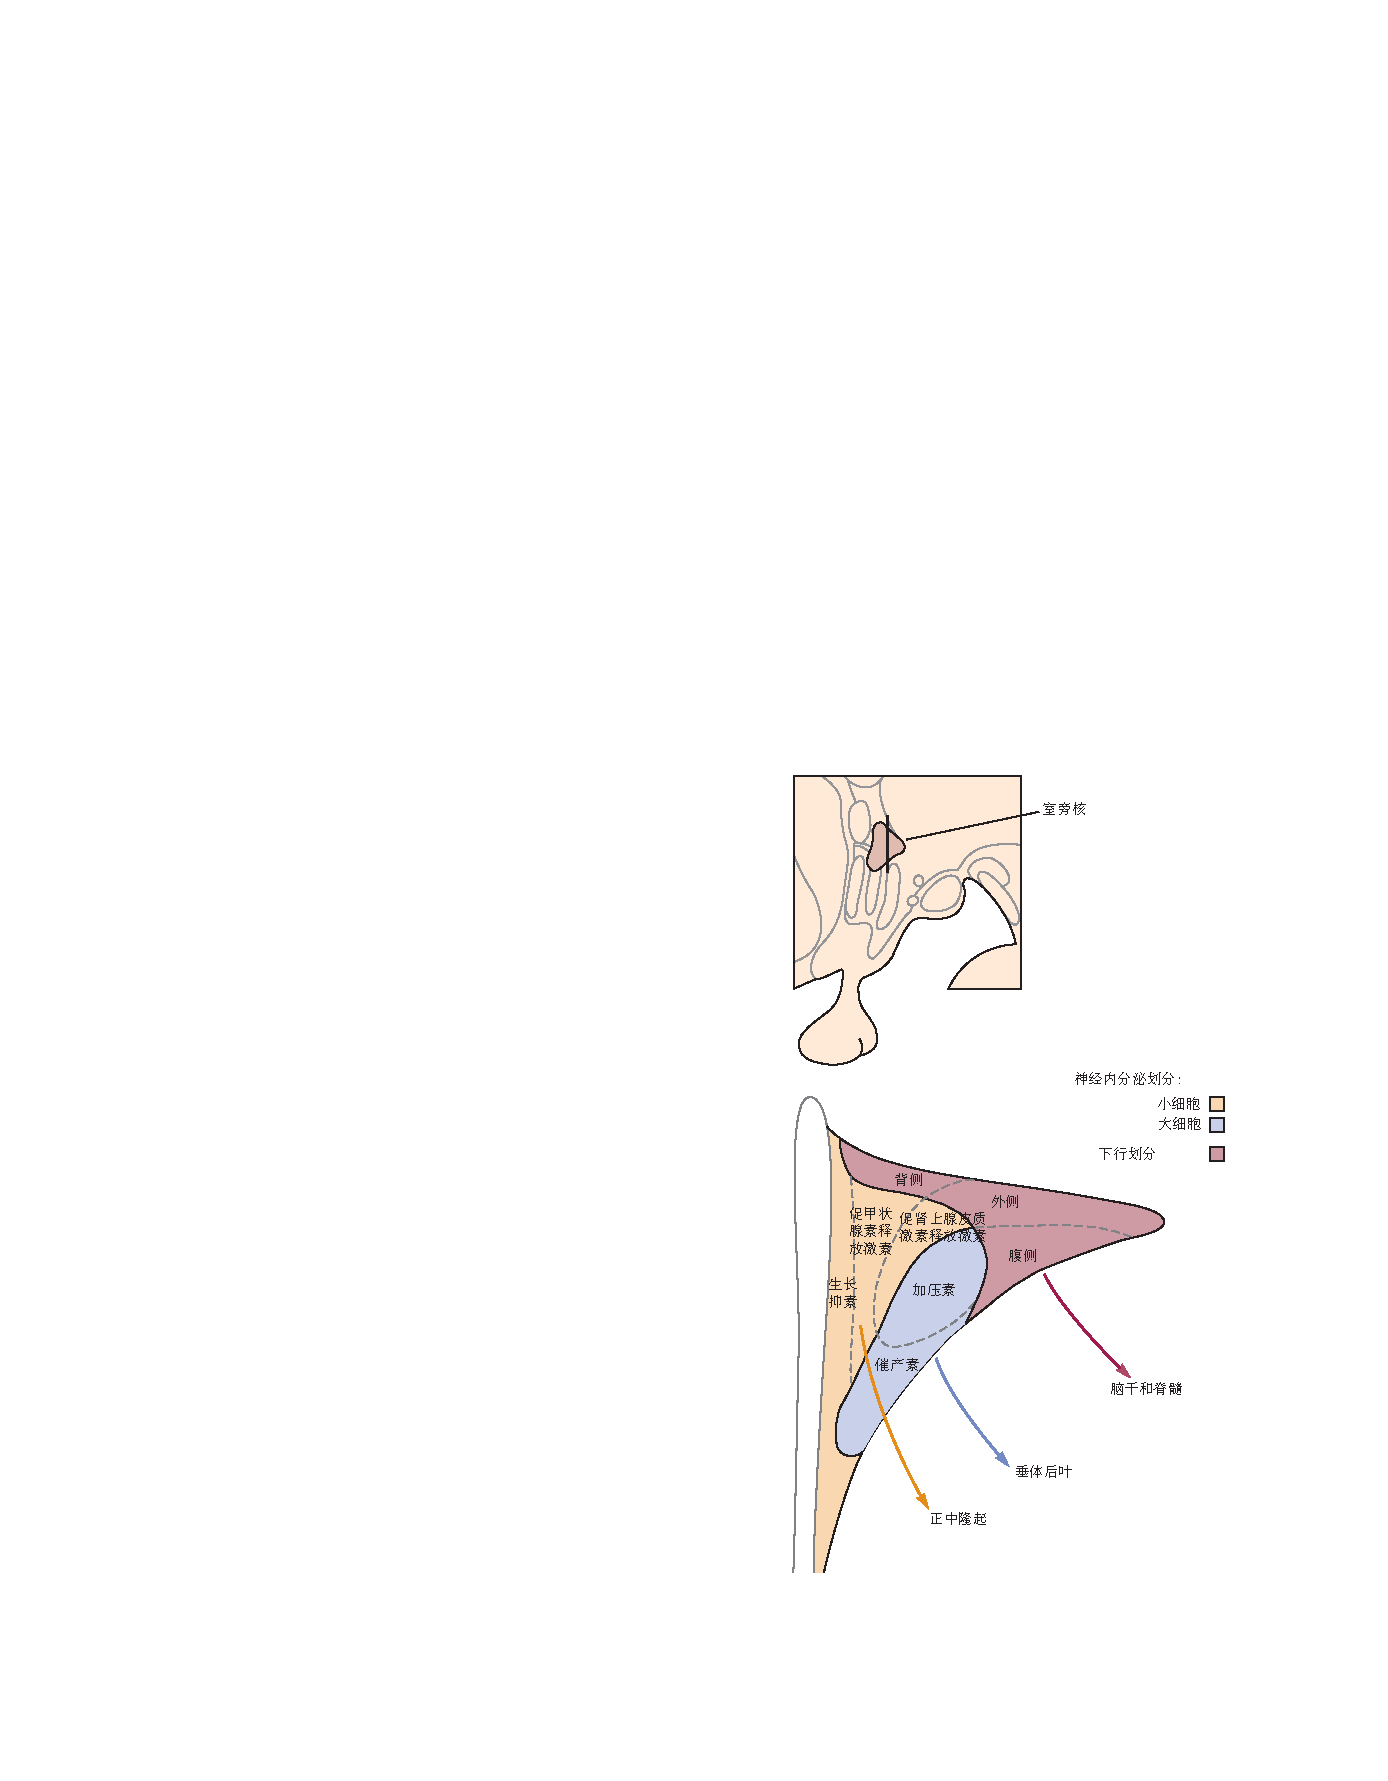
\includegraphics[width=0.54\linewidth]{chap41/fig_41_11}
	\caption{下丘脑的室旁核是神经内分泌、自动神经和感觉运动整合的缩影。
		显示了室旁核的三个结构功能分区。
		大细胞神经内分泌分裂包括两个不同但部分交叉的神经元池,它们通常释放\textit{加压素}或\textit{催产素}。
		它们的轴突穿过正中隆起的内部区域并终止于垂体后叶。
		另外两个大细胞加压素和催产素神经元群位于大脑底部的视上核中。
		小细胞神经内分泌分区包括三个主要的、独立的(虽然部分交叉)神经元池,它们控制垂体前叶激素的分泌。
		它们的轴突终止于正中隆起的外部区域,在那里它们释放肽类神经递质(\textit{生长抑素}、\textit{促甲状腺素释放激素}或\textit{促肾上腺皮质激素释放激素})进入垂体门静脉。
		下行部分有三个部分(背侧、外侧和腹侧)每个部分都包含投射到脑干和脊髓的按拓扑组织的常规神经元。
		如图~\ref{fig:41_10}~所示,它们的轴突终止于脑干中枢自动网络的许多部分、脊髓背角边缘区(lamina I)和脊髓三叉神经核,以及脑干网状结构和中脑导水管周围灰质的多个区域。
		下行部分调节自动流出(和流入)、伤害性信息的流入以及饮食行为。
		大细胞神经内分泌、小细胞神经内分泌、自动神经和行为反应的适当整合主要由外部输入介导,而不是由中间神经元或投射神经元的广泛循环轴突侧枝介导。
		循环类固醇和甲状腺激素也对室旁核中特定类型的神经元产生选择性作用。}
	\label{fig:41_11}
\end{figure}


\begin{figure}[htbp]
	\centering
	\includegraphics[width=0.65\linewidth]{chap41/fig_41_12}
	\caption{下丘脑通过神经内分泌神经元直接和间接地控制垂体。
		大细胞神经内分泌系统(蓝色)中的神经元将其轴突直接发送到垂体后叶(神经垂体),在那里它们将加压素肽和催产素释放到全身循环中。
		小细胞神经内分泌系统(黄色)中的神经元将其轴突发送到正中隆起和垂体柄的垂体门脉系统。
		如图~\ref{fig:41_11}~所示,门静脉将下丘脑激素(肽和多巴胺)输送到垂体前叶(腺垂体),在那里它们增加了五种经典类型的内分泌细胞的激素释放。
		神经内分泌神经元的输出在很大程度上受大脑其他区域输入的调节。}
	\label{fig:41_12}
\end{figure}


加压素和催产素是九个氨基酸的肽类激素。
与其他肽类激素一样,它们在细胞体中合成为较大的激素原(第~\ref{chap:chap16}~章),然后在沿着轴突向下移动到垂体后叶的释放位点之前在高尔基体运输小泡内被切割。
这些肽的基因具有相似的序列,可能是通过复制产生的。



\subsection{垂体前叶中的内分泌细胞响应下丘脑神经元释放的特定因子而分泌激素}

在 1950 年代,\textit{杰弗里$\cdot$哈里斯}提出垂体前叶或腺垂体是由下丘脑间接调节的。
如图~\ref{fig:41_12}~所示,他展示了将血液从下丘脑正中隆起输送到垂体前叶的垂体门静脉,以及从控制垂体前叶激素分泌的下丘脑神经元释放的转运因子。
在 1970 年代,\textit{安德鲁$\cdot$沙利}、\textit{罗杰$\cdot$吉莱明}和\textit{怀利$\cdot$瓦莱}确定了一组下丘脑肽激素的结构,这些激素控制垂体前叶中五种经典内分泌细胞类型的垂体激素分泌。
这些由下丘脑神经元释放到正中隆起的激素分为两类:释放激素和释放抑制激素。
只有一种垂体前叶激素,催乳素,主要处于抑制控制之下(由多巴胺介导)。


如图~\ref{fig:41_2}A~所示,下丘脑的小细胞神经内分泌运动区位于第三脑室壁的中心,包含投射到正中隆起并释放激素的神经元。
释放\textit{促性腺激素释放激素}的小细胞神经元是非典型的,因为它们散布在从内侧隔膜延伸到下丘脑内侧基底的连续体中。
它们由释放\textit{亲吻肽}的上游神经元控制。
如图~\ref{fig:41_2}~和图~\ref{fig:41_11}~所示,剩余的小细胞神经内分泌神经元位于室旁核和弓状核以及它们之间较短的脑室周围区域。


如图~\ref{fig:41_11}~所示,室旁核内和周围的不同神经元池释放\textit{促肾上腺皮质激素释放激素}、\textit{促甲状腺素释放激素}或生长抑素(或生长激素释放抑制激素)。
\textit{促肾上腺皮质激素释放激素}神经元控制垂体前叶\textit{促肾上腺皮质激素释放激素}的释放,\textit{促肾上腺皮质激素}又控制肾上腺皮质皮质醇(糖皮质激素)的释放。
因此,这个\textit{促肾上腺皮质激素释放激素}神经元池是所有中枢介导的糖皮质激素应激激素反应的“最终共同通路”。
弓状核包含两个小细胞神经内分泌神经元池。
一组释放\textit{生长激素-释放激素}和另一种抑制催乳素分泌的多巴胺。
一些多巴胺能神经元背侧分布至室旁核。


如图~\ref{fig:41_12}~所示,所有这些小细胞神经内分泌神经元的轴突在下丘脑-垂体束中行进,并终止于垂体柄的特殊近端,即正中隆起。
在那里,在中央隆起外部区域的毛细血管环区域中,轴突末端释放各种促生理性降压因子。
虽然中位隆起在大脑内,但它被认为在血脑屏障之外。
这是由于正中隆起毛细血管的开窗性质,它允许低生理性因子扩散到门脉循环中。
如图~\ref{fig:41_12}~和表~\ref{fig:41_3}~所示,正中隆起毛细血管环是垂体门静脉系统的近端,将因子输送到垂体前叶,在那里它们作用于五种内分泌细胞的同源受体。


\begin{table}[htbp]
	\caption{释放或抑制垂体前激素释放的下丘脑物质} \label{tab:41_3} \centering
	\begin{tabular}{ll}
		\toprule
		下丘脑物质 & 垂体前叶激素 \\
		\midrule
		\textit{释放:} &  \\
		促甲状腺素释放激素 & 促甲状腺激素、催乳素  \\
		促肾上腺皮质激素释放激素 & 促肾上腺皮质激素、$\beta$-促脂解素  \\
		促性腺激素释放激素 & 卵泡刺激素  \\
		生长激素-释放激素 & 生长激素  \\
		\textit{抑制:} &  \\
		催乳素分泌抑制因子 & 多巴胺  \\
		生长抑素 & 生长激素、促甲状腺激素  \\
		\bottomrule
	\end{tabular}
\end{table}



\section{专用的下丘脑系统控制特定的稳态参数}

\subsection{体温由\textit{正中视前核}中的神经元控制}

\textbf{体温反映热量产生和损失之间的平衡}

身体通过所有的放热生化反应和离子流动产生热量。
这些过程可以通过运动和颤抖(两者都会增加骨骼肌产热)、食物的消化和吸收(所谓的食物热效应)以及对棕色脂肪组织产热活动的交感神经刺激,大大高于基线水平,即静息代谢率(文本框~\ref{box:41_1})。


\begin{proposition}[棕色脂肪组织,生物能量学和交感神经驱动的产热] \label{box:41_1}
	
	\quad \quad 棕色脂肪组织是一种非常特殊的产热组织,在新生儿和小型哺乳动物中尤其丰富,但在成人中也有发现。
	它有丰富的血液供应,用于输送燃料和氧气以及散热,并被节后交感神经密集支配。
	棕色脂肪细胞是热量的产生者,存在于核心内部和其周围的浓缩沉积物中,也存在于较大的白色脂肪组织库中的分离细胞中。
	
	\quad \quad $\beta$-肾上腺素能受体的交感神经刺激激活\textit{解偶联蛋白1},\textit{解偶联蛋白1}是棕色脂肪细胞特有的线粒体质子转运蛋白。
	当被激活时,\textit{解偶联蛋白1}将质子穿过线粒体内膜“泄漏”到线粒体基质中,沿着质子电化学梯度向下。
	这使线粒体呼吸与\textit{二磷酸腺苷}的可用性脱钩,大大增加了燃料的氧化,重要的是,增加了热量的产生。
	
	\quad \quad 另一方面,运动和发抖通过使用\textit{三磷酸腺苷}进行工作来增加热量产生。
	由此产生的\textit{二磷酸腺苷}增加通过\textit{三磷酸腺苷}合酶激活质子转运到线粒体中,然后增加耦合的线粒体呼吸,燃料氧化,最终产生热量。
	
\end{proposition}


% The body loses heat by radiation
身体通过辐射、对流、传导(如果浸入冷水中)以及皮肤汗液或呼吸道水分的吸热蒸发(某些物种通过喘息加强这一过程)来散热。
除了产生热量外,对寒冷的防御反应还涉及交感神经介导的皮肤血管收缩和寒毛直立(鸡皮疙瘩)。
通过向皮肤输送较少的血液,血管收缩可以保持核心温度。
\textit{寒毛直立}通过在皮肤表面附近形成一层静止的空气来帮助隔离皮肤。
相反,防止过热的方法包括抑制激活皮肤血管扩张和棕色脂肪组织的交感神经通路。
自主的行为反应,如游泳或穿上毛衣,在体温调节中起着特别重要的作用。
它们通常在生理反应开始之前就开始了。
像口渴/饮水和饥饿/进食一样,响应冷或热挑战而产生的活动是有动机的行为。


\textbf{多处检测体温}

核心温度保持相对恒定。
另一方面,在外壳上,温度波动很大,因为外壳与外部环境相邻,它具有高表面质量比(在四肢有利于热量损失而不是热量产生的情况下),并且热挑战显著影响它的温血供应(当需要保存热量时减少;当需要散失热量时增加)。


大多数检测温度的初级传入在脊髓背根神经节中都有它们的细胞体。
检测有害温度的神经元是疼痛通路的一部分(第~\ref{chap:chap20}~章)。
它们的功能是通过促进戒断而不是调节体温来限制局部组织损伤。
对无害温度做出反应的神经元通常称为温度受体。
一些温度受体神经元的末端位于表皮下方的皮肤中,这些末端对外壳温度做出反应。
它们主要但不完全是冷反应。
其他温度受体神经元在大器官内和周围有末端,并对核心温度做出反应。
它们在很大程度上也有冷反应,但并非完全如此。
深层组织热受体神经元的纤维在内脏神经中移动,并且像壳中的热受体神经元一样,它们的细胞体位于背根神经节中。
此外,有的还走在迷走神经的传入神经中。
最后,下丘脑内侧视前区有温感神经元。


温度受体神经元用于检测温度变化的分子传感器是兴奋性\textit{瞬时受体电位}通道的一个子集。
不同的\textit{瞬时受体电位}通道响应不同的温度范围(第~\ref{chap:chap20}~章)。
最近的研究表明,特定\textit{瞬时受体电位}通道类型在上述三个部位以各种形式感知无害温度:
TRMP8 通道介导壳热受体神经元的冷感,TRPM2 通道介导体感热受体神经元和下丘脑前视神经元的暖感区域。


\textbf{多个热受体/热效应器回路控制温度}

非自主热调节由多传感器、多效应器体温调节系统控制。
来自壳和内脏的热信息通过其细胞体位于背根神经节中的初级传入神经上行。
它们投射到脊髓背角的二级神经元。
这些神经元通过脊髓丘脑束投射到\textit{臂旁外侧核},在那里神经元将冷感和暖感信息传递给下丘脑\textit{视前正中核}中的神经元。
冷感或暖感传入通路的激活会引起旨在升高或降低体温的适当生理反应。


\textit{视前正中核}中的神经元间接响应寒冷和温暖,通过内侧视前区、背内侧下丘脑和腹侧延髓中的苍白中缝传递传出信号,然后从那里到达脊髓中间外侧核中的交感节前神经元。
后一种神经元激发节后交感神经元,投射到血管、汗腺和毛囊的立肌,分别控制皮肤血流、出汗和\textit{寒毛直立},以及投射到棕色脂肪组织以控制产热。
此外,当脊髓腹侧角中的$\gamma$运动神经元被苍白中缝中的兴奋性神经元激活时,寒冷会引起颤抖(第~\ref{chap:chap32}~章)。
肌梭内梭内肌纤维由此产生的收缩激活了从纺锤到 $ \alpha $ 运动神经元的 IA 传入。
这种本体感受反馈增加了 $ \alpha $ 运动神经元的活动,以及它们进行有节奏活动爆发的倾向,导致肌肉张力增加和明显的颤抖。


控制自主体温调节行为的神经通路涉及相同的温度受体通路。
刺激\textit{视前正中核}内部和周围的暖敏神经元会引起显著的寻冷行为,减少热量产生并增加热量损失。
对体温的有意识感知依赖于相同的一级温度受体神经元,但传入通路发生分歧以激活背角中的二级神经元,后者直接或间接投射到丘脑腹内侧核中的神经元。
这些丘脑神经元投射到岛叶皮层。


从上面的讨论中可以清楚地看出,既没有体温设定点,也没有将体温维持在 37°C 的“恒温器”。
相反,如前所述,体温的明显设定点作为稳定点出现,由包含热受体和热效应器的多个感觉运动反馈回路控制。
这种多组分传入/传出系统能够如此有效地保持身体核心的温度非常恒定,这是进化的一项重大成就。


\textbf{控制温度的回路失调导致发烧}

过去,当体温调节的设定点观点占主导地位时,发烧被认为是体温设定点升高引起的,这一观点在各大医学教科书中仍然存在。
基于上述进展,现在认为发烧是通过传入/传出环路的调制引起的,特别是当它们穿过下丘脑视前区时。
前列腺素 E2 由炎性细胞因子对视前区内皮细胞的作用产生,可抑制\textit{视前正中核}中热激活的\textit{$\gamma$-氨基丁酸能}神经元,从而解除抑制促进皮肤血管收缩、棕色脂肪组织产热和颤抖的效应通路。
非甾体类抗炎药,如阿司匹林、布洛芬和对乙酰氨基酚,通过抑制下丘脑产生前列腺素 E2 来退烧。



\subsection{水平衡和相关的口渴驱动由终板、\textit{正中视前核}和穹隆下器官血管器官中的神经元控制}

\textbf{血液渗透压的变化导致细胞收缩或膨胀}

在渗透作用的驱动下,水可以自由穿过细胞膜。
这有许多重要的后果。
首先,由于其体积较大,细胞内隔室含有人体 2/3 的水分。
其次,如果血液渗透压与其正常值(290 \textit{毫渗透摩尔}/千克)发生变化,因为水分通过饮用获得或通过肾脏排泄和出汗流失,或者因为溶质通过进食(或通过饮用,例如海水)添加 —1000 \textit{毫渗透摩尔}/千克)(水会移动),所有隔室的渗透压都会平衡,包括细胞内的。


由于细胞内渗透活性分子的含量在短期内相对固定,血液渗透压升高会导致细胞收缩,反之,渗透压降低会导致细胞肿胀。
这对大脑特别危险,因为它被坚硬的头骨包裹着。
在极度高渗(水太少)的情况下,大脑会收缩,从头骨上拉开并撕裂血管。
低渗透压(水过多)会导致大脑肿胀,导致脑水肿、癫痫发作和昏迷。
为了防止此类事件发生,大脑会采取行动维持正常的渗透压。
它通过检测渗透压的变化然后调节饮水动机(口渴)和肾脏排泄水分的能力来实现这一点。


\textbf{当水分丢失或获得以及摄入食物时,渗透压会受到影响}

水是通过饮用获得的,在一定程度上是通过燃料的氧化(燃料 + O$_2$ → CO$_2$ + H$_2$O)获得的。
它以多种方式流失:通过呼吸(吸入干燥空气,排出潮湿空气)、通过胃肠道(尤其是出现腹泻时)、出汗和排尿。
进食还可以通过将水从血液转移到肠道以帮助消化以及在食物被分解和吸收时向血液中添加溶质来增加血液渗透压。


由于这些影响,控制饥饿和口渴的神经系统之间存在显著的相互作用。
例如,进食是一种如此重要的渗透压挑战,以至于脱水及其相关的高渗透压强烈抑制饥饿感(脱水诱发的厌食症)。
相反,进食本身的行为,即使在含水量正常的个体中,也会迅速刺激口渴,从而减轻预期的、进食引起的渗透压增加。


\textbf{垂体后叶释放的加压素调节肾的水排泄}

肾脏排泄水分的能力受到加压素的严格控制。
当它缺失时,人类可以排泄高达约 900 毫升/小时的尿液,而当它处于最高水平时,人类排泄量低至约 15 毫升/小时。
血管加压素通过增加肾脏对尿液的重吸收来减少水的排泄。


\textbf{渗透压由渗透压受体神经元检测}

大脑通过监测来自渗透压受体(响应渗透压的感觉神经元)的感觉输入来维持水平衡,渗透压受体反映了身体的水合状态。
渗透压受体神经元存在于外周和下丘脑内及周围的神经元上。
中枢渗透压受体监测全身渗透压,而外周渗透压受体监测肠道和相关结构内部和周围的渗透压。


\textbf{外周渗透压受体可以预测全身渗透压的变化}

关于外周渗透压的感觉信息使大脑能够先发制人地改变口渴和加压素分泌,从而预测和减轻未来全身渗透压的变化,例如饮酒时发生的减少或进食时发生的增加。
这种调节用于防止超过正常渗透压,否则当先前摄入的尚未影响全身渗透压的水从肠道缓慢吸收时会发生这种情况。
事实上,当一个脱水、高渗的个体摄入水时,口渴和加压素分泌迅速减少,远在全身渗透压下降之前。
外周渗透压受体的身份未知。


\textbf{中枢渗透压受体和传入/传出回路控制水平衡}

如图~\ref{fig:41_13}~所示,形成第三脑室前壁终板中的三个核在检测和响应全身渗透压紊乱方面起着关键作用。
从腹侧到背侧,它们是\textit{终板血管器官}、\textit{视前正中核}和\textit{穹窿下器}。
\textit{终板血管器官}和\textit{穹窿下器}是脑室周围器官,与前面讨论的正中隆起一样,它们位于血脑屏障之外。
正因为如此,这两个细胞核中的神经元可以快速检测到血液渗透压的变化以及无法穿过血脑屏障的血源性循环因子(一个重要的例子是血管紧张素 II)。


\begin{figure}[htbp]
	\centering
	\includegraphics[width=1.0\linewidth]{chap41/fig_41_13}
	\caption{神经和内分泌成分结合起来调节体液平衡。
		回路显示在大鼠大脑的矢状截面中。
		来自循环系统中的压力受体和口腔、喉咙和内脏中的感觉受体的信息通过舌咽(IX)和迷走神经(X)神经传递到孤束核和脑干尾部的邻近结构。
		激素\textit{血管紧张素} II 为大脑提供有关低血容量的额外信号。
		循环血管紧张素 II 被\textit{穹窿下器}中的受体感知; 
		\textit{穹窿下器}神经元投射到\textit{视前正中核}、\textit{下丘脑室旁核}、\textit{视上核}和\textit{终板血管器官}。
		血液的渗透压由投射到\textit{视前正中核}、\textit{下丘脑室旁核}和\textit{视上核}的\textit{终板血管器官}内和附近的受体感知。
		\textit{下丘脑室旁核}和\textit{视上核}细胞核中的神经分泌细胞触发垂体后叶释放加压素,从而减少肾脏的水排泄\cite{swanson2000cerebral}。}
	\label{fig:41_13}
\end{figure}


与这种排列一致,\textit{终板血管器官}和\textit{穹窿下器}中的渗透压受体神经元与\textit{视前正中核}中的神经元建立了广泛的联系。
虽然\textit{视前正中核}神经元本身不直接感知渗透压,但它们通过来自\textit{终板血管器官}和\textit{穹窿下器}的转发器间接响应渗透压。
虽然\textit{终板血管器官}和\textit{穹窿下器}中的所有神经元似乎都致力于调节水平衡,但如前所述,\textit{视前正中核}中的一些神经元参与调节体温、心功能和睡眠。
水平衡或体温的调节由\textit{视前正中核}中的形态特异性神经元亚群执行。


来自所有三个终板核的神经元向\textit{下丘脑室旁核}和视上核中的分泌性加压素神经元发送密集的兴奋性投射。
如下所述,这三个终板核也能引起口渴。


中枢渗透压受体,可能还有外周渗透压受体,通过响应细胞体积的变化来检测渗透压的变化。
收缩或膨胀分别增加或减少它们的阳离子渗透性,导致燃烧速率增加或减少。


血管内容量减少(例如,由于急性失血)也能有效刺激口渴和加压素分泌。
肾脏检测到低血容量,从而增加肾素的分泌。
肾素是一种蛋白酶,可将循环血管紧张素原转化为\textit{血管紧张素} I。
然后\textit{血管紧张素} I 在肺中被血管紧张素转换酶进一步切割,生成\textit{血管紧张素} II。
\textit{血管紧张素} II 直接激发\textit{穹窿下器}神经元,并通过\textit{视前正中核}中的转发器驱动加压素神经元和假定的口渴神经元。


口渴由\textit{终板血管器官}、\textit{视前正中核}和\textit{穹窿下器}中的神经元控制

与加压素分泌一样,所有三个终板结构都参与产生口渴的动机状态,即寻找和摄取水的欲望。
所有三个结构的损伤完全阻断了脱水和\textit{血管紧张素} II 引起的口渴,以及加压素的分泌。
另一方面,对这些结构的电刺激会引起饮水行为。
\textit{穹窿下器}和\textit{视前正中核}中兴奋性谷氨酸能神经元的激活会在几秒钟内诱导一只饱水小鼠的强烈饮水。


因此,\textit{穹窿下器}和\textit{视前正中核}中的兴奋性神经元以及\textit{终板血管器官}中的兴奋性神经元具有显著的诱发口渴的能力。
重要的是,诱导的行为是特定的(只发生饮水)。
值得注意的是,驱动这种行为的兴奋性\textit{穹窿下器}神经元与脱水激活并表达\textit{血管紧张素} II 受体的\textit{穹窿下器}神经元亚群相同。
这些神经元刺激口渴的下游通路目前尚不清楚。


\textit{穹窿下器}中的口渴神经元和\textit{视上核}和\textit{下丘脑室旁核}中的加压素神经元的活动分别响应于感官线索(例如饮水或进食)而迅速减少或增加,这些感官线索可预测未来的稳态紊乱。
这种快速调节的发生与系统渗透压的任何变化无关,因此与反馈无关;
因此,它是前馈控制的一个例子。
这种前馈调节的可能功能是预测干扰,采取先发制人的纠正措施,从而大大减少或消除它们的影响。


总之,多年的研究已经形成了一个清晰的模型。
脱水(缺水)会增加\textit{穹窿下器}和\textit{终板血管器官}中神经元的活性,并通过来自\textit{穹窿下器}和\textit{终板血管器官}的中继增加\textit{视前正中核}中的神经元活性,并且这种活性的增加会增强口渴和加压素分泌。
正如我们将看到的,一个类似的通用系统,但具有不同的神经结构,控制基于热量不足的饥饿和能量代谢调节。



\subsection{能量平衡和相关的饥饿驱动由弓状核中的神经元控制}

与温度和水平衡一样,能量平衡由来自身体的反馈信号调节,这些反馈信号调节关键的下丘脑神经元的活动,然后启动生理和行为的适应性变化。
然而,能量平衡的调节在重要方面有所不同。


首先,监测到的反馈信号很多,而且在许多情况下,与关键参数能量平衡只有非常间接的关系。
这种反馈的例子包括来自肠道的神经和激素信号、来自脂肪细胞的瘦素、来自胰腺 $ \beta $ 细胞的胰岛素以及血液中的代谢物水平。
这与监测温度调节和水平衡的单一、直接感测信号形成鲜明对比。
其次,能量可以储存为脂肪。
可蓄积的能量非常高,足以满足一个人挨饿一个多月的能量需求。
相比之下,热量和水不会被储存。
因此,生物体有一个“能量缓冲”,可以在长期缺乏时存活下来。


第三,由于储存有好处,与温度和水平衡相反,能量平衡的调节是不对称的,因为低能量储存受到非常积极的防御,而高能量储存只受到非常微弱的防御,因此在热量密集、可口食物的社会中肥胖症的患病率很高。
第四,能量储存可能是一种负担,当能量储存过多时,它会促进肥胖、糖尿病、心脏病和癌症等疾病的发生。
最后,在调节能量平衡的回路中,神经肽起着非常重要的作用。


\textbf{当能量摄入超过消耗时,脂肪就会储存起来}

根据热力学第一定律,以脂肪形式储存的卡路里等于摄入的卡路里减去消耗的卡路里。
虽然获得能量的方法只有吃一种,但消耗能量的方法有很多种。


大多数能量都被基本生命功能所需的生化反应所消耗。
由于这些过程一直在运行,因此这种“强制性能量消耗”是固定的,不受监管。
然而,另外两种类型的能量消耗却截然不同;
一种是自主的身体活动,而另一种是非自主的,由棕色脂肪组织的交感神经刺激和颤抖引起。
交感神经控制的能量消耗,通常称为适应性产热,由大脑控制。
它的功能是响应温度和能量存储的扰动。


\textbf{能量的摄入和消耗通常是匹配的}

对于大多数人来说,身体脂肪储存随着时间的推移相对恒定。
因此,摄入的卡路里大致等于消耗的卡路里。
一个简单的计算证明了这一点。
一个中年人平均每天消耗 3,392 千卡(千卡对应于常用术语“卡路里”)。
在一年的过程中,这个典型的人增加了 350 克脂肪(相当于每天 9 千卡脂肪)。
因此,平均而言,每天必须额外消耗 9 千卡才能实现这一收益。
这是典型糖果的4\%的能量或步行约 150 米消耗的能量。
因此,摄入和消耗之间的不匹配(9 千卡)很小(仅占总能量消耗的 0.27\%)。


这种紧密匹配是强大的稳态机制的结果,该机制利用身体的反馈来调节摄入和消耗。
正如温度和渗透压的调节一样,体重的恒定性以及摄入量和消耗量之间的紧密匹配与任何特定的“设定点”无关。
相反,这种非凡的控制是多个传入/传出反馈回路的紧急稳定点。


\textbf{肥胖是由基因和最近的生活方式改变引起的}

上述传入/传出反馈回路失调会导致肥胖。
虽然一些肥胖病例是由于稳态调节所需的已知基因突变引起的,但大多数肥胖病例的原因不明。
其中,许多可能是由于多重突变,其中许多是未表征的。
由于近年来西方社会的肥胖发病率大幅增加,其速度快到不能归因于新的突变,因此饮食和身体活动的改变也必须发挥重要作用。
为在狩猎采集者中实现能量平衡而进化的稳态系统很可能被丰富、可口、热量密集的食物所淹没。


但即使在我们现代的致胖环境中,脂肪储存仍然存在很大差异:
只有 41\% 到 70\% 的脂肪储存个体差异可归因于遗传因素。
因此,遗传易感性和环境共同导致肥胖。
有趣的是,迄今为止发现的许多易感基因位点都涉及影响大脑功能的基因。


\textbf{多重传入信号控制食欲}

影响能量平衡的主要传入信号可分为两大类。
(1)来自胃肠道细胞的短期信号报告肠道中食物的状态。
除了一种信号外,所有这些信号都随着进食而增加,并起到终止进餐的作用;
生长素释放肽是个例外,它会随着禁食而增加并刺激饥饿感。
(2)长期信号报告能量储备(即脂肪储存)的状态。 
这些包括胰腺激素胰岛素和脂肪细胞激素瘦素,两者的释放都与脂肪储存成比例。
如图~\ref{fig:41_14}A~所示,它们的水平,尤其是瘦素水平,会告知大脑脂肪储存是否充足。


\begin{figure}[htbp]
	\centering
	\includegraphics[width=0.79\linewidth]{chap41/fig_41_14}
	\caption{神经和内分泌成分结合起来调节能量平衡。 
		A. 短期信号。
		在进餐期间,来自肠道的\textit{胆囊收缩素}刺激迷走神经的感觉纤维,从而促进饱腹感(进餐终止)。
		同样由肠道释放的\textit{胰高糖素样肽-1}和\textit{多肽 YY}似乎对迷走神经的感觉纤维和大脑中的神经元起作用。
		迷走神经感觉纤维,连同来自肠道和口腔感觉信息的交感神经纤维,汇聚在\textit{孤束核}中。
		进餐前,胃中生长素释放肽的释放达到峰值,向大脑中的神经元提供血源性信号。
		\textit{胆囊收缩素}促进饱腹感,而生长素释放肽促进进食。
		长期信号。
		瘦素和胰岛素是告知大脑脂肪储存状态的体液信号。
		瘦素在脂肪储存细胞中产生,而胰岛素在胰腺中产生。
		这两种激素都被下丘脑弓状核中的受体以及\textit{孤束核}中的受体感知。
		瘦素和胰岛素减少食物摄入并增加能量消耗。
		B. 弓状核中合成\textit{刺鼠相关肽}(\textit{促食欲相关肽})、\textit{前阿黑皮素}和\textit{囊泡谷氨酸转运体2型}的神经元投射到\textit{下丘脑室旁核},其中他们控制饥饿和饱腹感。
		促进饱腹感的\textit{前阿黑皮素}神经元释放经过处理的\textit{前阿黑皮素}肽,\textit{$\alpha$-黑素细胞刺激素},它与\textit{下丘脑室旁核}神经元上的\textit{黑素皮质素受体4}结合。
		这些神经元的激活会导致饱腹感。
		相反,促进饥饿的\textit{促食欲相关肽}神经元释放两种抑制性递质,\textit{$\gamma$-氨基丁酸}和\textit{神经肽Y},以及\textit{黑素皮质素受体4}拮抗剂\textit{促食欲相关肽}。
		它们的综合作用是抑制表达\textit{黑素皮质素受体4}的神经元,从而引起饥饿。
		表达\textit{黑素皮质素受体4}的神经元还接收来自另一群弓状神经元\textit{囊泡谷氨酸转运体2型}神经元的直接兴奋性输入,这也促进饱腹感。
		\textit{$\alpha$-黑素细胞刺激素}与\textit{黑素皮质素受体4}的结合通过两种机制引起饱腹感:通过直接激活 \textit{下丘脑室旁核}-\textit{黑素皮质素受体4}神经元和通过上调从弓状\textit{囊泡谷氨酸转运体2型}神经元到 \textit{下丘脑室旁核}-\textit{黑素皮质素受体4}神经元的兴奋性传递(蓝色箭头)。
		最后,\textit{下丘脑室旁核}-\textit{黑素皮质素受体4}神经元投射到外侧臂旁核,在那里它们促进饱腹感。}
	\label{fig:41_14}
\end{figure}


\textit{来自肠道的信号触发膳食终止。}
在进食期间,当食物进入胃和肠时,身体膨胀会增加对拉伸敏感的迷走神经传入神经的放电。
此外,肠道内分泌细胞对食物的化学检测会刺激\textit{胆囊收缩素}、\textit{胰高糖素样肽-1}和\textit{多肽 YY}等激素的分泌。
这些反应具有三个主要功能。


首先,它们引起幽门括约肌收缩,幽门括约肌是胃和肠之间的瓣膜。
这限制了食物的进一步通过,防止小肠超载。
其次,肠道激素刺激胆汁和酶分泌到肠腔中以帮助消化。
第三,迷走神经传入和肠道激素减少随后的食物摄入,导致进餐终止(饱腹感)。
肠道激素主要通过刺激局部迷走神经传入神经末梢来实现这一点,这反过来又会刺激\textit{孤束核}尾部区域的神经元。


其中两种激素\textit{胰高糖素样肽-1}和\textit{多肽 YY}也可以直接刺激大脑中的神经元。
\textit{孤束核}中激活的神经元直接或通过\textit{臂旁外侧核}中的中继投射到前脑中的神经元,包括杏仁核和下丘脑。
表达\textit{降钙素基因相关肽}的\textit{臂旁外侧核}中的神经元是参与饱腹感的重要中继之一。
然后这些回路导致进餐终止。


当食物被吸收时,血糖升高会刺激 $ \beta $ 细胞释放胰岛素和胰岛淀粉样多肽。
胰岛淀粉样多肽随后激发极后区(位于\textit{孤束核}正上方的血脑屏障外的脑室周围器官)中的神经元。
循环胰淀素在饭后几分钟内增加,减少随后的食物摄入。


\textit{生长激素释放肽}由胃中的内分泌细胞释放。
与上述因素不同的是,它在进食前分泌量高,进餐时分泌量下降。
它可能在开始进餐的过程中起发挥作用。
事实上,生长素释放肽是唯一已知的会增加饥饿感并因此增加进食量的系统性因素。
它会激发多个部位的神经元,包括弓状核中与\textit{刺鼠相关肽}神经元(见下文)。
\textit{生长激素释放肽}的生理意义尚不清楚,因为其基因的缺失似乎不会影响饥饿感。


% Blood Glucose and Insulin Affect Appetite
\textit{血糖和胰岛素影响食欲。}
葡萄糖由外周、后脑和下丘脑的神经元感知。
尽管葡萄糖传感似乎在能量平衡的日常调节中没有发挥作用,但检测和应对危险的低血糖水平(葡萄糖减少症)是大脑的一项重要功能。
启动了两种适应性反应:
(1)强烈的葡萄糖缺乏饥饿,至少部分是由于与\textit{刺鼠相关肽}神经元的间接激活,以及(2)胰高血糖素、肾上腺素和皮质类固醇的分泌,它们刺激肝葡萄糖的产生。
荷尔蒙反应是由交感神经流出增加以及与压力相关的\textit{促肾上腺皮质激素释放激素}通路激活引起的(第~\ref{chap:chap61}~章)。
氨基酸也可以被感知,从而调节能量平衡和饮食选择,后者确保摄入足够数量和质量的蛋白质。


另一方面,胰岛素被认为是脂肪储存增加的信号。
胰岛素的主要功能是控制血糖,刺激其分泌。
胰岛素通过将其驱入肌肉和脂肪细胞并减少肝脏产生的胰岛素来降低血糖。
随着脂肪储存量的增加,其执行此操作的能力会降低(一种称为胰岛素抵抗的现象)。
因此,较高的脂肪储存会增加基础和膳食刺激的胰岛素分泌,以努力克服抵抗力并使葡萄糖正常化。
脂肪储存介导的胰岛素水平升高会抑制下丘脑中的神经元,尤其是弓状核,这被认为可以减少饥饿感。


% The Fat Cell Hormone Leptin Signals the Brain
\textit{脂肪细胞激素瘦素向大脑发出有关脂肪储存的信号,并影响饥饿和能量消耗。}
1949 年,缅因州杰克逊实验室的科学家注意到“一些非常丰满的小老鼠”的出现。
这种肥胖是由基因突变引起的,他们将其命名为肥胖基因(ob)。
16 年后,他们发现了另一种肥胖突变,即\textit{糖尿病}基因(db)。
ob/ob 和 db/db 小鼠的极度肥胖是由强烈的摄食和减少的棕色脂肪产热引起的。
基于一系列的共生实验,\textit{道格拉斯$\cdot$科尔曼}提出 ob/ob 小鼠缺乏循环饱腹感因子,而 db/db 小鼠缺乏其受体。


% In a tour-de-force positional cloning effort
在\textit{杰弗里$\cdot$弗里德曼}和\textit{鲁道夫$\cdot$利贝尔}领导的一项杰出定位克隆工作中,ob 基因定位于 6 号染色体上的一个小区域。
\textit{弗里德曼}和他的实验室随后锁定并鉴定了 ob 基因。
重新命名为瘦素基因,它编码瘦素,一种由脂肪细胞分泌的 167 个氨基酸的蛋白质,与脂肪储存的大小成比例。
用瘦素治疗 ob/ob 小鼠可以治愈它们的肥胖症。
db 基因在几年后被发现,正如\textit{科尔曼}预测的那样,它编码了瘦素受体,并被发现在下丘脑的神经元中表达。
它是一种白介素 6 型 I 类细胞因子受体,通过激活 JAK2/STAT3 信号通路产生抗肥胖作用。


后来人们对瘦素有了很多了解。
首先,患有瘦素或其受体基因缺陷的人类,如突变小鼠,会严重肥胖;
因此,瘦素的功能是高度保守的,这种突变极为罕见。
其次,患有常见肥胖症的人的瘦素循环水平非常高,瘦素是脂肪储存量增加的副产品。
这一发现最初导致了一种观点,后来受到质疑,即“普通”肥胖是由对瘦素作用的抵抗引起的。
第三,节食减少了脂肪储备,大幅降低了瘦素水平。
这种减少很有趣,因为禁食会导致许多适应性反应,这些反应也见于缺乏瘦素的小鼠和人类:饥饿、低能量消耗、生育能力下降和其他神经内分泌反应改变。
事实上,禁食个体恢复正常瘦素水平可以逆转或改善许多禁食效应。
因此,瘦素的主要功能是在其水平较低时发出信号,表示脂肪储存不足。


这些低瘦素水平会带来关键的适应性反应,例如增加饥饿感、减少交感神经介导的产热作用(以保存有限的燃料储存)、降低生育能力(在无法满足其需求时防止怀孕)等。
根据这种观点,瘦素的信号动态范围从禁食时的极低水平(表明脂肪储存量过低)延伸到在饱食、非肥胖个体中发现的水平(表明脂肪储存量充足)。
高于此水平可能会产生一些抑制肥胖的效果,但如果存在这种效果,则非常微弱。
因此,能量平衡的防御是不对称的,即对低储量强,对高储量弱。
一个推论是肥胖的人没有瘦素抵抗。
相反,他们只是瘦素水平超过了最大有效浓度。


\textbf{\textit{前阿黑皮素}、\textit{促食欲相关肽}和\textit{黑素皮质素受体4}神经元是传入/传出回路中的关键节点}

神经元特异性操作技术揭示了弓状核中控制能量平衡的两个拮抗神经元群:
如图~\ref{fig:41_14}B~所示,一个表达\textit{刺鼠相关肽}(\textit{促食欲相关肽}),另一个表达前体多肽原\textit{前阿黑皮素}。
\textit{前阿黑皮素}神经元减少饥饿感并刺激交感神经驱动的能量消耗;
\textit{促食欲相关肽}神经元则相反。
\textit{前阿黑皮素}神经元释放加工过的肽$\alpha$-促黑素细胞激素(\textit{$\alpha$-黑素细胞刺激素}),它激活\textit{黑素皮质素受体4}(一种 G 蛋白偶联受体)。


控制饥饿的下游表达\textit{黑素皮质素受体4}的神经元位于\textit{下丘脑室旁核}内。
当这些\textit{黑素皮质素受体4}神经元被\textit{前阿黑皮素}传入神经释放的\textit{$\alpha$-黑素细胞刺激素}兴奋时,饥饿感就会减少。
\textit{下丘脑室旁核}-\textit{黑素皮质素受体4}“饱腹感神经元”是谷氨酸能的;
它们通过兴奋性投射到\textit{臂旁外侧核}来减少饥饿感。


控制能量消耗的表达\textit{黑素皮质素受体4}的神经元是脊髓中的交感神经节前神经元。
除了\textit{下丘脑室旁核}之外,\textit{前阿黑皮素}神经元还投射到这些部位,增加了交感神经驱动的能量消耗。


如图~\ref{fig:41_14}B~所示,\textit{促食欲相关肽}神经元部分地通过对抗\textit{前阿黑皮素}神经元的动作来增加饥饿感。
它们释放三个因子:\textit{促食欲相关肽},一种\textit{黑素皮质素受体4}的反向激动剂,以及神经肽 Y 和 \textit{$ \gamma $-氨基丁酸},两种抑制性递质。
\textit{促食欲相关肽}神经元投射到并抑制\textit{下丘脑室旁核}-\textit{黑素皮质素受体4}饱腹感神经元,并直接抑制\textit{前阿黑皮素}神经元。
此外,弓状\textit{促食欲相关肽}神经元的不同子集投射到其他部位,包括外侧下丘脑和终纹床核。
这些位点在被\textit{促食欲相关肽}输入抑制时,也可以刺激饥饿感。


如图~\ref{fig:41_14}B~所示,弓状核中的第三组神经元表达\textit{囊泡谷氨酸转运体2型},释放谷氨酸,并与\textit{前阿黑皮素}神经元并行作用以诱导饱腹感。
与\textit{前阿黑皮素}神经元一样,与\textit{促食欲相关肽}神经元相反,它们会激发\textit{下丘脑室旁核}-\textit{黑素皮质素受体4}饱腹感神经元。
\textit{下丘脑室旁核}-\textit{黑素皮质素受体4}神经元中的\textit{$\alpha$-黑素细胞刺激素}/\textit{黑素皮质素受体4}信号通过两种机制引起饱腹感:
通过直接激活\textit{下丘脑室旁核}\textit{黑素皮质素受体4}饱腹感神经元和通过突触后易化上调从\textit{囊泡谷氨酸转运体2型}神经元到 \textit{下丘脑室旁核}\textit{黑素皮质素受体4} 神经元的兴奋性传递。


许多令人信服的发现支持\textit{前阿黑皮素}、\textit{促食欲相关肽}和 \textit{下丘脑室旁核}\textit{黑素皮质素受体4} 饱腹感神经元在调节食物摄入方面的重要性。
首先,禁食会激活\textit{促食欲相关肽}神经元并抑制\textit{前阿黑皮素}神经元,而进食或瘦素治疗则相反。
下游 \textit{下丘脑室旁核}-\textit{黑素皮质素受体4}饱腹感神经元被禁食抑制,被进食兴奋。
其次,\textit{前阿黑皮素}蛋白或\textit{黑素皮质素受体4}的遗传缺陷会导致大量肥胖。
第三,小鼠\textit{促食欲相关肽}神经元的基因消融会导致饥饿,而\textit{促食欲相关肽}神经元的刺激会迅速导致极度摄食,即使在热量充足或饱食的小鼠中也是如此。
最后,一些发现表明 \textit{下丘脑室旁核}-\textit{黑素皮质素受体4}饱腹感神经元是\textit{促食欲相关肽}和\textit{前阿黑皮素}神经元的重要下游目标。
最值得注意的是在\textit{下丘脑室旁核}中缺乏\textit{黑素皮质素受体4}神经元的基因工程小鼠中明显的摄食过多和肥胖的发展,以及在\textit{下丘脑室旁核}中\textit{促食欲相关肽}末端的光遗传学刺激后诱导强烈进食,这抑制了饱腹感神经元。


令人惊讶的是,预测未来食物摄入的环境线索会抑制\textit{促食欲相关肽}神经元。
事实上,在具有高\textit{促食欲相关肽}神经元活性的禁食小鼠中,单独提供食物而不摄入会减少\textit{促食欲相关肽}神经元放电。
这大致类似于加压素分泌和口渴神经元活动的快速前馈抑制(如前所述)。
因此,除了从身体接收到强烈的自下而上的反馈信号外,促进饥饿的\textit{促食欲相关肽}神经元还接收来自环境的自上而下的前馈信息。
此输入的功能尚不清楚,但它可以作为限制未来摄入过多卡路里的预期信号,或者如下文所述,它可以作为激励进食的奖励相关信号。


最后,目前尚不清楚\textit{促食欲相关肽}和\textit{前阿黑皮素}神经元→ \textit{下丘脑室旁核}通路调节饥饿的完整通路。
它很可能通过许多突触的中继,影响控制奖励和感知通路中的神经元活动。
之所以如此,是因为在禁食状态下,食物和预测食物的线索都更有价值,也更有可能成为关注的焦点。
当神经信息从下丘脑中高度特异性缺陷调节的稳态神经元流向伏隔核和皮层中的“非特异性”奖励和感知通路时,如何保留对于特定目标(在本例中为食物)的特异性,这是饥饿和口渴等动机行为的最大谜团之一。
该解决方案可以为药物成瘾等动机行为障碍提供线索。


\textbf{心理学概念被用来解释动机驱动,例如饥饿}

在一种简化的行为刺激-反应观点中,人们可能会假设缺水或能量缺乏(刺激)的神经检测与饮水或进食(反应)的运动通路相关联,因此类似于膝跳牵张反射( 第~\ref{chap:chap3}~章)。
然而,情况并非如此,因为可用于获取食物的反应都是由缺乏刺激引起的,这些反应非常多样和复杂,以至于它们无法硬连线。
事实上,动物可以完成无数复杂的操作性学习任务以获得水或食物奖励。


理解动机驱动力的挑战是设计一个模型来解释剥夺状态诱导非常多变和复杂的行为的能力,同时保持完全针对一个目标。 两个引人注目的理论是相关的。
根据激励动机理论,食物和水的缺乏会增加其奖励价值。
减少驱动力理论认为,缺乏会产生厌恶状态,而认为这种状态的解决会激发行为。
值得注意的是,这两种观点并不相互排斥,在某些方面可能是同一问题的两面。


激励动机:禁食增加食物的奖励价值。
激励动机理论是理论家多年的工作,最近由\textit{弗雷德里克$\cdot$托茨}和\textit{肯特.贝里奇}完善。
考虑进食和饥饿感。
简而言之,食物被视为天生有益。
通过习得的联想,与获取食物相关的线索和任务也变得有益;
如图~\ref{fig:41_15}A~所示,以这种方式,学习了各种复杂的行为反应。


\begin{figure}[htbp]
	\centering
	\includegraphics[width=0.86\linewidth]{chap41/fig_41_15}
	\caption{关于禁食如何促进进食的两种理论。 
		A. 激励动机。
		食物本质上是有回报的,不同的食物有不同的回报值(生菜:低,冰淇淋:高)。
		通过习得的联想,预测食物的线索变得有益。 进食(吃饱)与禁食状态设置了增益,决定了食物和食物线索的奖励程度。
		禁食会大大增加,而饱足状态会降低奖励值。
		B. 减少驱动。
		饥饿的感觉令人厌恶。
		进食可以减少这种厌恶状态。
		与这一理论一致,促进饥饿的\textit{刺鼠相关肽}(\textit{促食欲相关肽})神经元的实验刺激令人厌恶,而刺激下丘脑\textit{黑素皮质素受体4}神经元(位于\textit{促食欲相关肽}和阿黑皮质素原的下游)的促进饱腹感的室旁核神经元[\textit{前阿黑皮素}] 在一只饥饿的老鼠身上会产生一种愉快的感觉。}
	\label{fig:41_15}
\end{figure}


该理论假定剥夺状态增加了食物和相关线索和任务的奖励价值(即,它们的激励显著性)。
因此,在禁食期间,奖励值增加,所有食物以及与食物相关的提示和任务都获得了极大的奖励。
饭后,奖励值降低,只有最可口的食物,例如冰淇淋,仍然有足够的奖励可以吃。
神经科学家的任务是确定剥夺如何增加奖励价值。
\textit{促食欲相关肽}在饱腹的小鼠中,\textit{促食欲相关肽}神经元的实验激活显著增加了食物的奖励价值。
值得注意的是,食物的奖励价值增加到与禁食时相同的极高水平。


减少驱动力:\textit{促食欲相关肽}饥饿神经元的活动可能令人厌恶。
正如我们从个人经验中所知,脱水和热量不足造成的行为状态,即口渴和饥饿,是令人不愉快的。
它最初是在多年前提出的,减少这些状态可以缓解这种不适,是有益的,因此会激发饮水和进食。
最近,如图~\ref{fig:41_15}B~所示,\textit{斯科特$\cdot$斯特内森}的团队为该模型的修改版本提供了令人信服的新支持。
通过使用行为条件反射范式,如位置偏好测试,他们发现饱腹小鼠中\textit{促食欲相关肽}\textit{促食欲相关肽}神经元的光遗传学激活是令人厌恶的。
当同样的小鼠在食物剥夺状态(与\textit{促食欲相关肽}神经元活动增加相关)下进行研究时,它们会做出在早期条件反射中降低\textit{促食欲相关肽}神经元活动的行为,简而言之,它们表现得好像有动力关闭\textit{促食欲相关肽}神经元诱导的厌恶状态。
\textit{穹窿下器}中的口渴神经元也获得了类似的结果。


为了进一步支持这一观点,下游\textit{下丘脑室旁核}-\textit{黑素皮质素受体4}饱腹感神经元的光遗传学激活在热量剥夺的小鼠中是情绪积极的(即小鼠喜欢它),但在饱食小鼠中则不然。
因此,在饥饿时引起饱腹感是令人愉快的。
总的来说,这些发现为以下观点提供了强有力的证据:
稳态缺陷令人不愉快,厌恶状态是由缺陷反应性稳态神经元的激活引起的,并且当受到缺陷诱导的厌恶状态的折磨时,动物会做出与它们相关的行为。


这个模型解释了为什么节食如此困难。
它会产生一种厌恶、不愉快的状态,只能通过进食来缓解。
最后,\textit{促食欲相关肽}神经元活动响应于预测食物的感官线索的快速减少,以及这应该引起的厌恶状态的缓解,可以作为激励追求目标(食物)的奖励“教学信号”。



\section{下丘脑中的性二态区域控制着性、攻击性和育儿}

现在我们转向非稳态但受下丘脑控制的行为,涉及感觉线索和来自身体的信号(即性腺类固醇)之间的整合,并且对物种的生存至关重要。


雄性和雌性在性、攻击性和养育行为方面存在差异。
这些差异在动物中尤其显著,例如在小鼠中,它们显然是天生的(即不需要事先训练)。
这些差异分别包括雄性和雌性的交配和脊柱前凸;
领土相关行为,例如雄性的标记和侵略;
以及在与后代打交道时,雌性倾向于养育,而男性倾向于采取攻击性行为。
这些性二态行为的潜在能力是胚胎发生过程中性类固醇对大脑作用的产物(第~\ref{chap:chap51}~章)。
成人特定性别行为的完全实现也需要成人水平的性腺类固醇。
性染色体特异性基因,除了导致男性性别决定的 Sry 之外,以及以性二态方式印记的基因,也巧妙地调节独立于性腺类固醇的性别特异性行为。
最终,行为本身是由来自环境的线索触发的,例如信息素。


下丘脑的两个区域与这些行为的控制密切相关,即\textit{视前区}和\textit{下丘脑腹内侧核的腹侧侧面}。
这两个位点都是性二态的:\textit{视前区}在男性中包含更多的神经元,而\textit{下丘脑腹内侧核的腹侧侧面}在女性中包含更多的孕激素表达神经元。
这些部位紧密相连,它们从下丘脑外的其他两个性二态区域接收强烈输入:
\textit{终纹床核后侧的内侧分裂}和\textit{内侧杏仁核}。



\subsection{性行为和攻击性受视前下丘脑区和腹内侧下丘脑核亚区的控制}

脑损伤研究表明,性二态性大脑区域(附属嗅球、\textit{终纹床核后侧的内侧分裂}、\textit{内侧杏仁核},尤其是\textit{视前区}和\textit{下丘脑腹内侧核的腹侧侧面})在性别特异性行为中发挥重要作用。
如图~\ref{fig:41_16}~所示,这些区域中的神经元高度相互关联,位于参与检测和响应信息素(\textit{终纹床核后侧的内侧分裂}和\textit{内侧杏仁核})的通路的下游,表达性激素受体,并且除了\textit{下丘脑腹内侧核的腹侧侧面}中的神经元外,还表达芳香酶。
\textit{视前区}和\textit{下丘脑腹内侧核的腹侧侧面}中的神经元向外侧\textit{中脑导水管周围灰质}区域发出强烈投射,该区域被认为可以调节和协调性和攻击性行为的运动和自动方面。


\begin{figure}[htbp]
	\centering
	\includegraphics[width=0.95\linewidth]{chap41/fig_41_16}
	\caption{性二态神经结构包含高度互连的行为回路。
		调节两性二态行为的下丘脑和杏仁核广泛相互关联。
		这些区域处理信息素信息,每个区域内的成年神经元亚群表达性激素受体;
		其中一些区域(蓝色)内的神经元也表达芳香化酶。}
	\label{fig:41_16}
\end{figure}


\textit{下丘脑腹内侧核的腹侧侧面}在控制性二态行为中起着关键作用。
雄性小鼠\textit{下丘脑腹内侧核的腹侧侧面}神经元的放电率在交配或对雄性入侵者的攻击期间增加。
刺激这些神经元会触发对入侵者雄性和非典型雄性攻击目标的强烈攻击行为,例如阉割的雄性、雌性,甚至是橡胶手套!
沉默这些神经元可以消除对雄性入侵者的攻击行为。
此外,刺激表达雌激素受体的\textit{下丘脑腹内侧核的腹侧侧面}神经元子集会引起性行为(增加)或攻击性,具体取决于激活的神经元数量及其激活程度:较低水平的激活会导致增加,而较高水平会导致攻击性。
与这些结果一致,相关孕激素受体表达\textit{下丘脑腹内侧核的腹侧侧面}神经元的基因消融导致雄性性行为和攻击性丧失以及雌性性行为丧失。
因此,很明显,表达\textit{下丘脑腹内侧核的腹侧侧面}的类固醇受体中的性神经元在驱动雄性和雌性的性行为以及雄性的攻击性方面起着关键作用。



\subsection{视前下丘脑区控制父母行为}

养育父母的行为是后代生存的关键。
雄性啮齿动物和雌性表现出截然不同的行为模式。
雄性对后代可能是养育或敌对,甚至到了杀婴的地步,这取决于它们将后代视为自己的还是其他雄性的。
另一方面,雌性老鼠通常是在养育。


小鼠幼崽与友好的成年雌性和雄性小鼠(但不是敌对的成年雄性小鼠)之间的社会互动会诱导\textit{视前区}中表达甘丙肽神经元亚群的活动。
这些后代激活的神经元在很大程度上不同于通过交配激活的\textit{视前区}神经元。
表达甘丙肽的\textit{视前区}神经元的基因消融会阻止养育父母的行为,甚至会导致雌性对其后代产生异常的攻击性。
另一方面,雄性通常对无关的幼崽极度敌对,刺激这些甘丙肽阳性神经元会减少攻击性并诱导养育幼崽梳理毛发。
因此,\textit{视前区}中的神经元除了控制性行为本身外,还在确保性行为果实的存活方面发挥作用。



\section{要点}

1. 下丘脑与自动神经和神经内分泌运动系统通过诱导适应性行为协调和控制\textit{内稳态};
通过控制腺体、平滑肌、心肌和脂肪细胞;
并通过垂体释放激素。 


2. 体温、体液和电解质平衡以及血压的稳态控制允许生物体在恶劣的环境条件下发挥作用。


3. 感应温度、渗透压、血压和体脂的反馈回路对于稳态控制至关重要。
多个反馈通知的感觉传入/传出效应器控制回路的联合作用导致紧急稳定点。


4. 形态特异性下丘脑神经元将特定的内感受性感觉反馈与控制适应性行为和生理反应的输出联系起来。
除了反馈之外,这些特定于模式的神经元还接收有关未来预期稳态挑战的前馈信息。


5. 自动运动系统包含位于靠近脊柱或嵌入外周目标的交感神经节、副交感神经节和肠神经节中的神经元。
自动神经元的功能子集选择性地支配由平滑肌、心肌、腺上皮细胞和脂肪细胞组成的效应组织。


6. 交感神经元因运动和压力而被激活。
副交感神经和交感神经通常具有拮抗功能,但通常协同作用。
肠系统协调胃肠道的蠕动收缩与粘膜功能和局部血流。


7. 控制交感神经和副交感神经流出的神经节前神经元位于脊髓和脑干。


8. 乙酰胆碱、去甲肾上腺素和神经肽协同递质在自动运动系统中充当突触信号分子。
自动神经节中的兴奋性快速突触传递由作用于烟碱受体的乙酰胆碱介导。
神经节中的 G 蛋白偶联受体介导额外的突触前和突触后兴奋和抑制作用。
G 蛋白偶联受体介导自动神经效应器连接处的递质作用。 


9. 神经内分泌系统通过垂体将下丘脑与身体的各种生理反应联系起来。
垂体后叶包含下丘脑轴突末端,可将两种神经激素释放到血液中:加压素刺激肾脏对水的重吸收,而催产素控制子宫收缩和乳汁释放。
垂体前叶含有内分泌细胞,可根据下丘脑神经元释放的因子分泌激素。
这些垂体前叶激素控制甲状腺、肾上腺皮层分泌糖皮质激素、性腺分泌性类固醇、泌乳和线性生长。


10. 多部位检测体温,包括外周、主要器官内部和周围、大脑。
体温的恒定性由多个热受体-传入/热效应器-传出控制回路维持。


11. 终板中的一些神经元因脱水和血管内容量减少而被激活。
在这些缺乏状态下感知的关键参数分别包括渗透压和血管紧张素 II 水平。
当这些神经元被激活时,它们会引起口渴并从垂体后叶释放加压素。
加压素的释放也通过预测未来渗透压紊乱的线索以前馈方式快速调节。 


12. 能量平衡涉及短期和长期反馈信号。
来自肠道的短期信号调解饱腹感,从而终止进餐。
由肠道内分泌细胞释放的\textit{胆囊收缩素}在饱腹感中起着关键作用。
一个关键的长期信号是瘦素,脂肪细胞分泌的瘦素与脂肪储存量成正比。
当脂肪储存量低时,随之而来的低水平瘦素会向大脑发出信号,引发饥饿状态并减少能量消耗,从而补充脂肪储存量。 


13. 瘦素在抵御低脂肪储存方面比在抵抗肥胖方面更有效。 


14. 下丘脑中表达\textit{前阿黑皮素}-、\textit{促食欲相关肽}- 和\textit{黑素皮质素受体4}的神经元是控制能量平衡的传入/传出回路中的关键节点。
发出饱腹感信号的神经元被促进饱腹感的\textit{前阿黑皮素}神经元激活,并被促进饥饿的\textit{促食欲相关肽}神经元抑制。


15. 当神经信息从下丘脑中高度特异性缺陷调节的稳态神经元流向伏隔核和皮层中的“非特异性”奖励和感知通路时,如何保留给定目标(例如食物)的特异性,这是饥饿和口渴等动机行为的最大谜团之一。
解决这个问题可以为药物成瘾等动机行为障碍提供线索。 


16. 瘦素部分通过激活\textit{前阿黑皮素}神经元和抑制\textit{促食欲相关肽}神经元来调节饥饿和能量消耗。
促进饥饿的\textit{促食欲相关肽}神经元也通过预测未来能量平衡变化的线索以前馈方式快速调节。


17. 饥饿等动机驱动可以通过两种机制来解释:
缺乏状态(饥饿)会增加食物的奖励价值,或者缺乏会产生厌恶状态,而厌恶状态的解决会激发行为。 


18. 下丘脑的性二态区域控制性行为和攻击性。
两性异形视前区的神经活动控制着父母的行为。
成人特定性别行为的完全实现也需要成人水平的性腺类固醇。

